\section*{Chapter 4: Results and Discussion}
\phantomsection \setcounter{section}{4} \setcounter{subsection}{0}
\addcontentsline{toc}{section}{\textit{Chapter 4: Results and Discussion}}

This chapter presents the experimental results of the proposed hybrid model and three baseline models across all classification tasks, followed by error analysis, attention visualisation, statistical significance testing, and a comparison with published literature.

All results in this chapter come from strict recording-level 10-Fold cross-validation with no data leakage. Metrics are reported as mean $\pm$ standard deviation across the 10 folds.

\subsection{Classification Performance across All Tasks}

\subsubsection{Binary Classification: Normal (Z+O) vs.\ Seizure (S)}

Table~\ref{table:binary_results} presents the binary classification results. All four models achieve accuracy above 98.8\%, reflecting the substantial signal-level differences between normal EEG ($<$200~$\mu$V amplitude) and seizure activity ($>$1000~$\mu$V). This ceiling effect is consistent with findings reported in the literature: Thara et al.\ \cite{thara2019} reported 99.08\% under an 80/20 segment-level split, while Ullah et al.\ \cite{ullah2018} reported up to 99.1\% using a pyramidal CNN.

\begin{table}[H]
  \centering
  \begin{spacing}{1.35}
  \caption{Binary Classification Results --- Normal (Z+O) vs.\ Seizure (S)}\vspace{0.7em}
  \label{table:binary_results}
    {\small
    \begin{tabular}{|>{\raggedright\arraybackslash}p{7.0cm}|>{\raggedright\arraybackslash}p{2.8cm}|>{\raggedright\arraybackslash}p{2.8cm}|}
    \hline
    \textbf{Model} & \textbf{Accuracy (\%)} & \textbf{F1 Score (\%)} \\
    \hline
    SVM + Wavelet Packet & 99.67 ($\pm$1.00) & 99.66 ($\pm$1.01) \\
    \hline
    Pure 1D-CNN & 98.86 ($\pm$1.91) & 98.84 ($\pm$1.95) \\
    \hline
    Pure Bi-LSTM + Attention & 99.48 ($\pm$1.29) & 99.47 ($\pm$1.29) \\
    \hline
    \textbf{CNN + Bi-LSTM + Attention (Ours)} & \textbf{99.67 ($\pm$0.85)} & \textbf{99.66 ($\pm$0.86)} \\
    \hline
    \end{tabular}
    }
  \end{spacing}
\end{table}

The hybrid model ties with SVM at 99.67\% accuracy but achieves the lowest reported variance ($\pm$0.85\% vs.\ $\pm$1.00\%), indicating the most consistent cross-fold performance in the current runs.

Figure~\ref{fig:tc_binary_combined} shows the combined 10-fold training curves. The model converges rapidly --- most folds reach near-perfect validation accuracy within 20 epochs, with early stopping terminating training shortly after. The tight clustering of fold curves reflects the consistency of this task.

\begin{figure}[H]
\centering
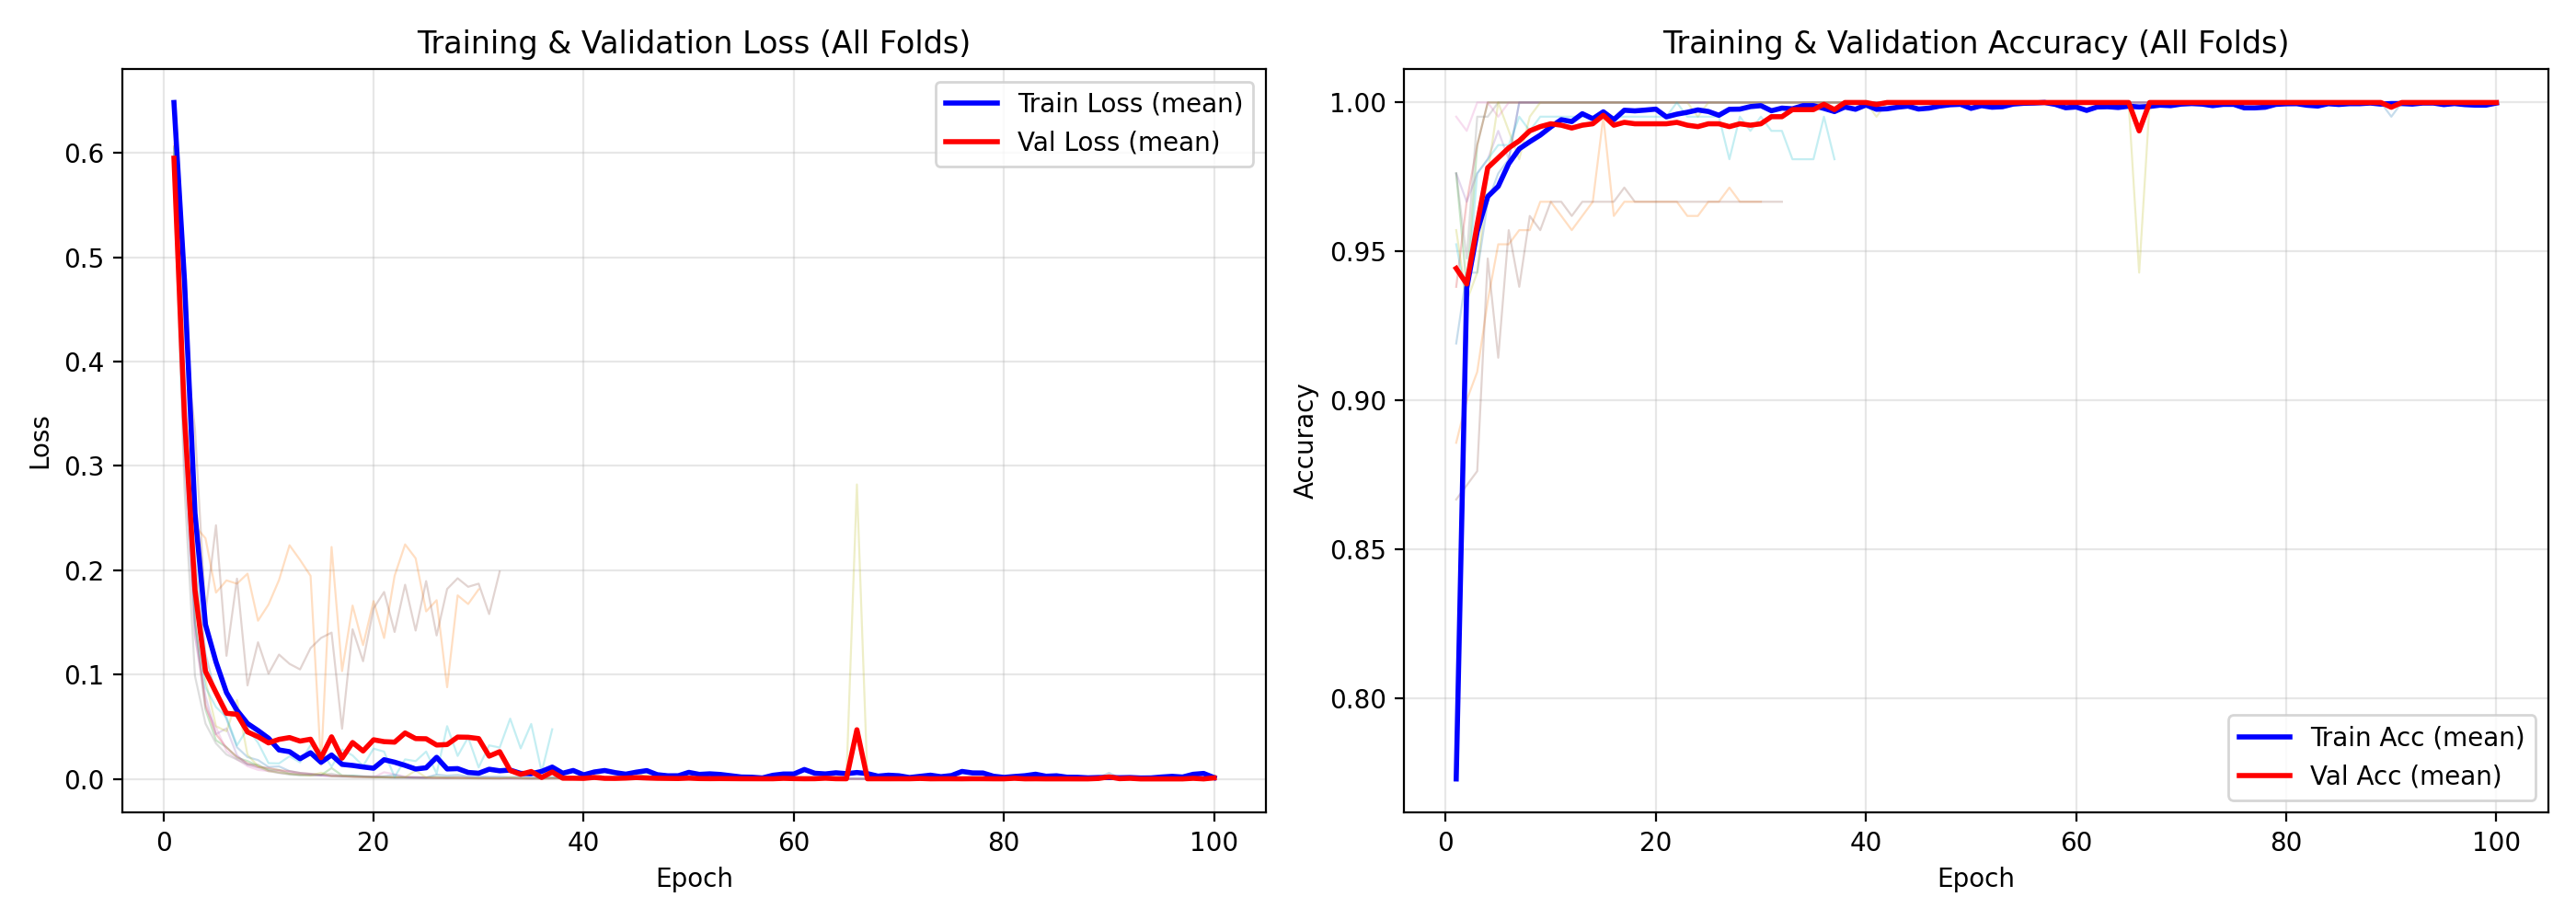
\includegraphics[width=\textwidth]{figures/training_curves_binary_hybrid.png}
\caption{Combined 10-fold training curves for binary classification. Light lines: individual folds; bold line: mean.}
\label{fig:tc_binary_combined}
\end{figure}

Figure~\ref{fig:tc_binary_fold} compares the best and worst folds. Fold~1 converges to 100\% within 15 epochs. Fold~6 is the lowest-performing fold (97.1\%), where validation loss remains slightly elevated.

\begin{figure}[H]
\centering
(a) Fold 1 --- best performance (100\%)\\[0.2em]
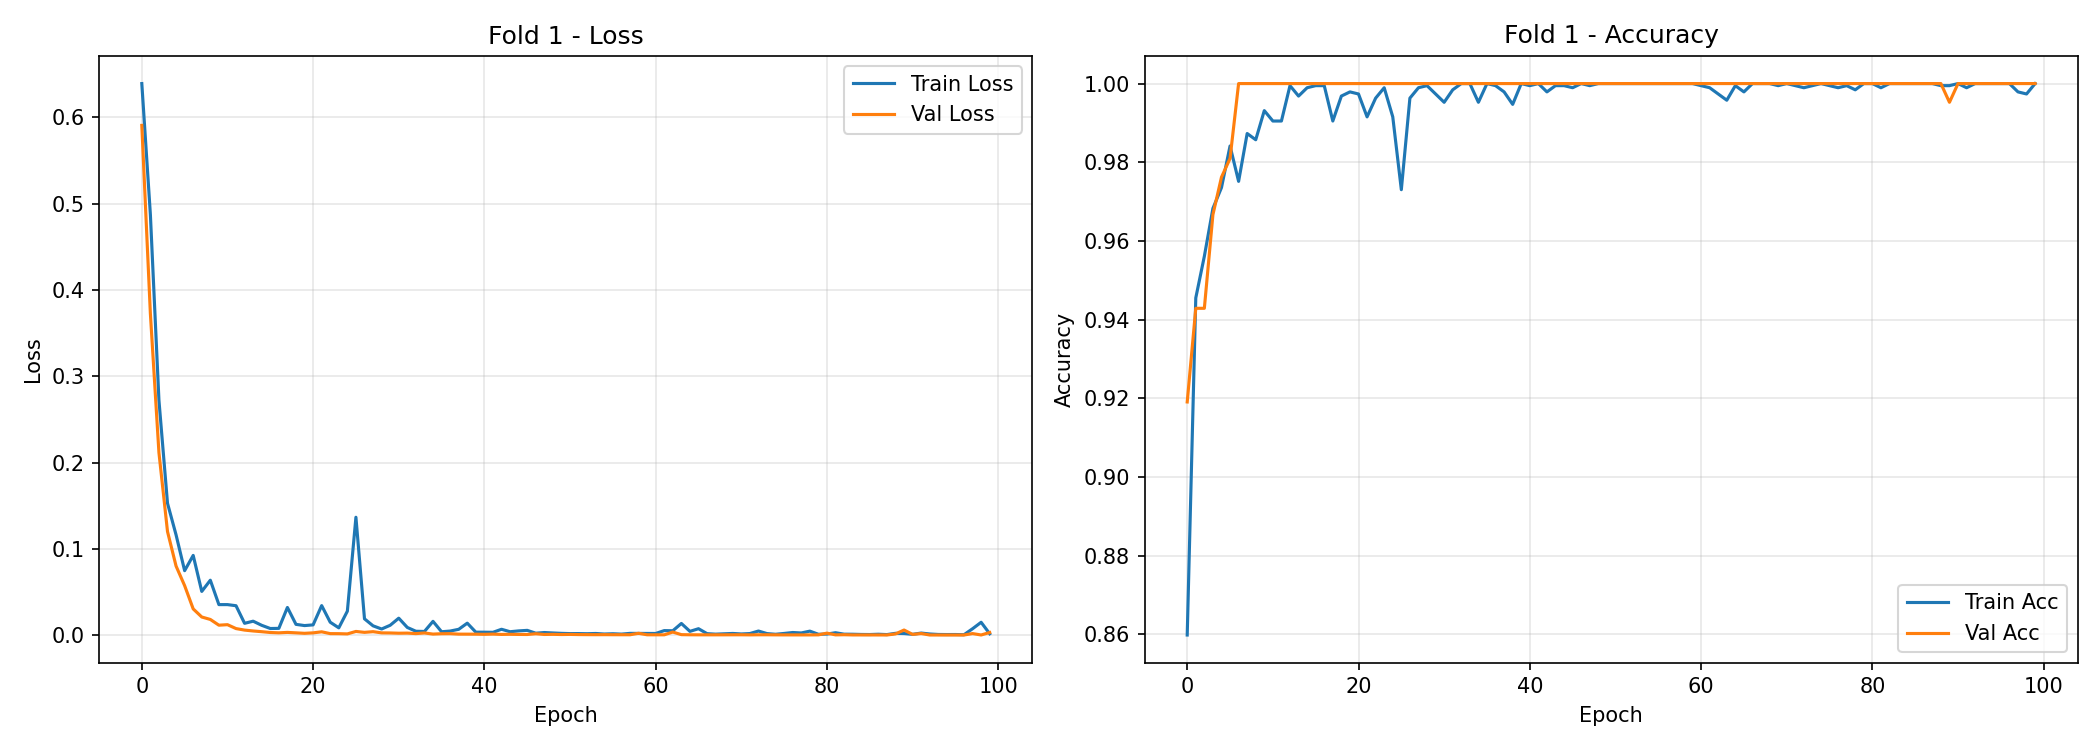
\includegraphics[width=0.88\textwidth]{figures/tc_binary_fold1.png}
\vspace{0.15cm}

(b) Fold 6 --- lowest performance (97.1\%)\\[0.2em]
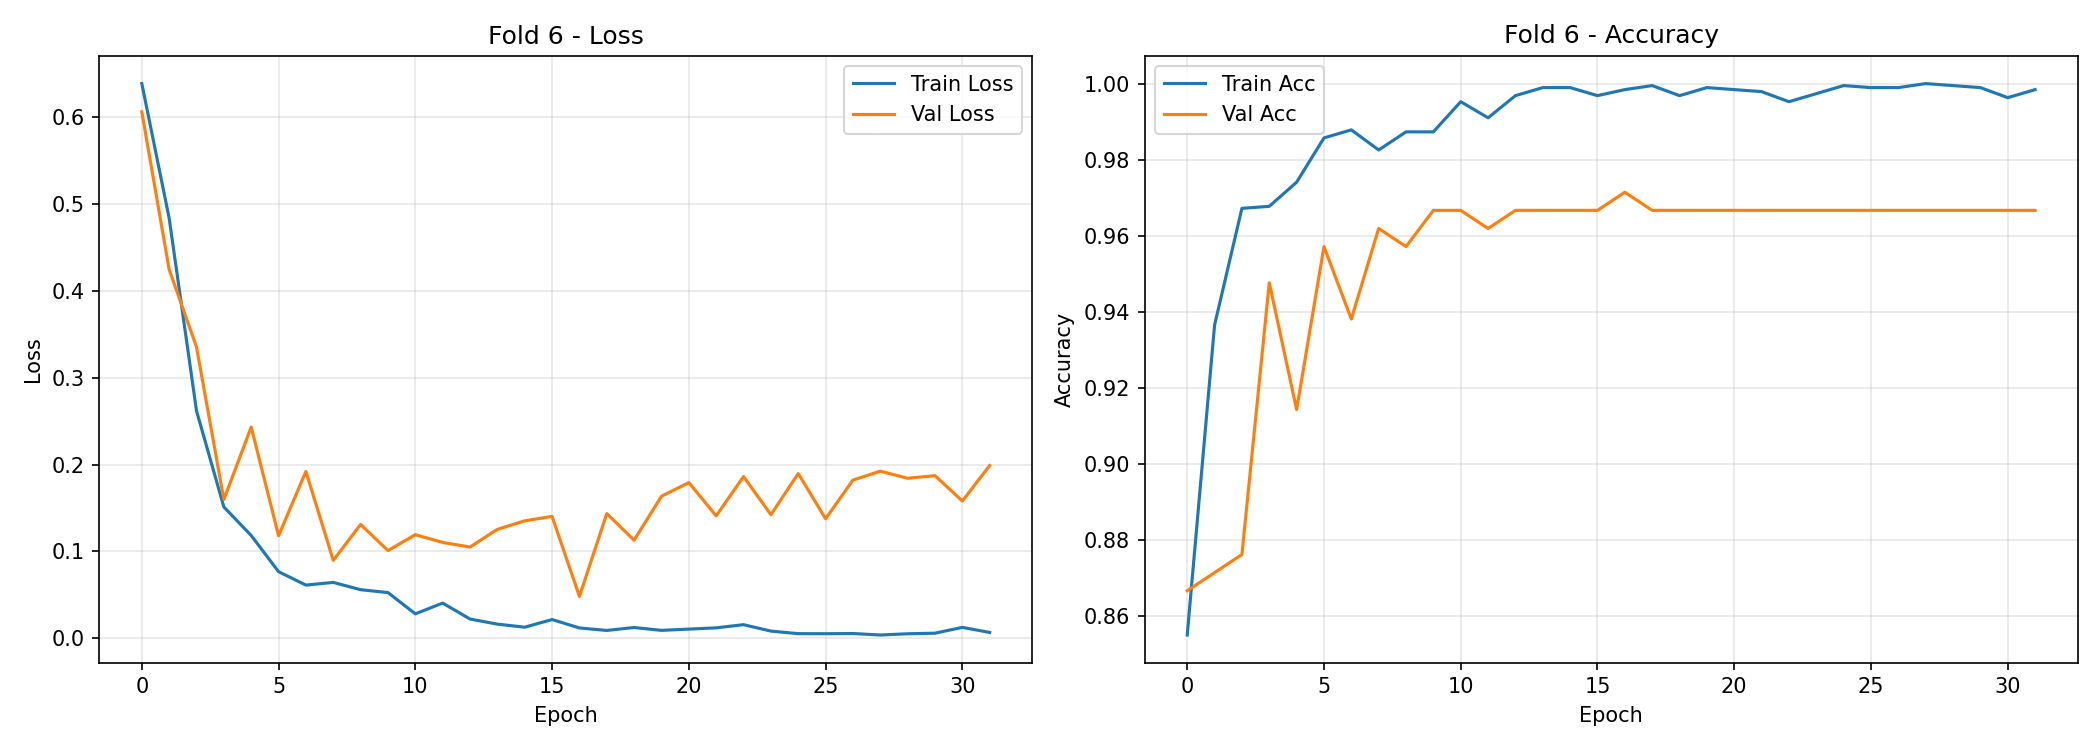
\includegraphics[width=0.88\textwidth]{figures/tc_binary_fold6.png}
\caption{Individual fold training curves for binary classification, showing the best and worst folds.}
\label{fig:tc_binary_fold}
\end{figure}

\subsubsection{Three-class Classification: Normal vs.\ Inter-ictal vs.\ Seizure}

Table~\ref{table:three_results} shows the three-class results. The introduction of the inter-ictal class increases task difficulty, as inter-ictal EEG shares some morphological features with both normal and seizure recordings.

\begin{table}[H]
  \centering
  \begin{spacing}{1.35}
  \caption{Three-class Classification Results --- Normal vs.\ Inter-ictal vs.\ Seizure}\vspace{0.7em}
  \label{table:three_results}
    {\small
    \begin{tabular}{|>{\raggedright\arraybackslash}p{7.0cm}|>{\raggedright\arraybackslash}p{2.8cm}|>{\raggedright\arraybackslash}p{2.8cm}|}
    \hline
    \textbf{Model} & \textbf{Accuracy (\%)} & \textbf{F1 Score (\%)} \\
    \hline
    SVM + Wavelet Packet & 94.20 ($\pm$2.44) & 94.19 ($\pm$2.44) \\
    \hline
    Pure 1D-CNN & 97.14 ($\pm$1.84) & 97.11 ($\pm$1.86) \\
    \hline
    Pure Bi-LSTM + Attention & 92.80 ($\pm$5.99) & 92.74 ($\pm$6.12) \\
    \hline
    \textbf{CNN + Bi-LSTM + Attention (Ours)} & \textbf{97.69 ($\pm$2.17)} & \textbf{97.68 ($\pm$2.17)} \\
    \hline
    \end{tabular}
    }
  \end{spacing}
\end{table}

The hybrid model achieves the highest accuracy at 97.69\%, outperforming SVM by +3.49\% and Pure Bi-LSTM by +4.89\%. The Pure Bi-LSTM exhibits notably high variance ($\pm$5.99\%), suggesting that raw-signal sequence modelling without CNN-based local feature preprocessing is less stable in this setting. The Pure CNN performs competitively at 97.14\%, only 0.55\% below the hybrid model.

Combined 10-fold curves were not generated for the three-class task during the original experiments. Figure~\ref{fig:tc_three_fold} shows representative folds. Folds~1 and~5 converge above 97\% validation accuracy, while Folds~9 and~10 plateau at 94--95\%, pulling the overall mean to 97.69\%.

\begin{figure}[H]
\centering
(a) Fold 1 --- converges above 97\%\\[0.1em]
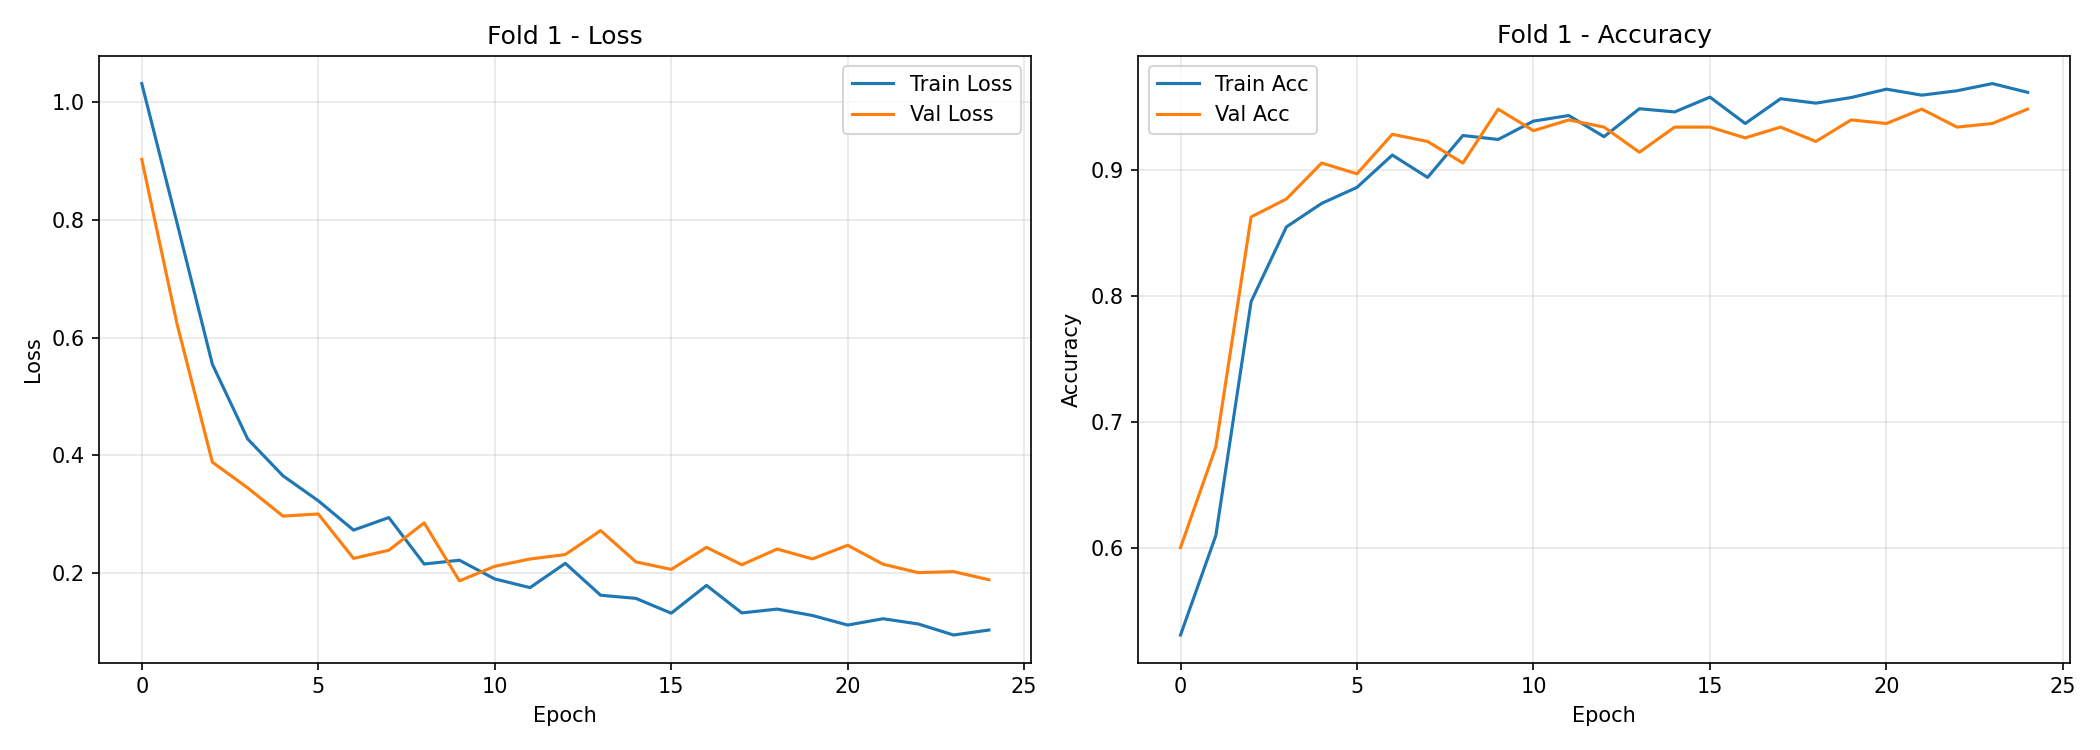
\includegraphics[width=0.82\textwidth]{figures/tc_three_fold1.png}
\vspace{0.1cm}

(b) Fold 5 --- converges above 97\%\\[0.1em]
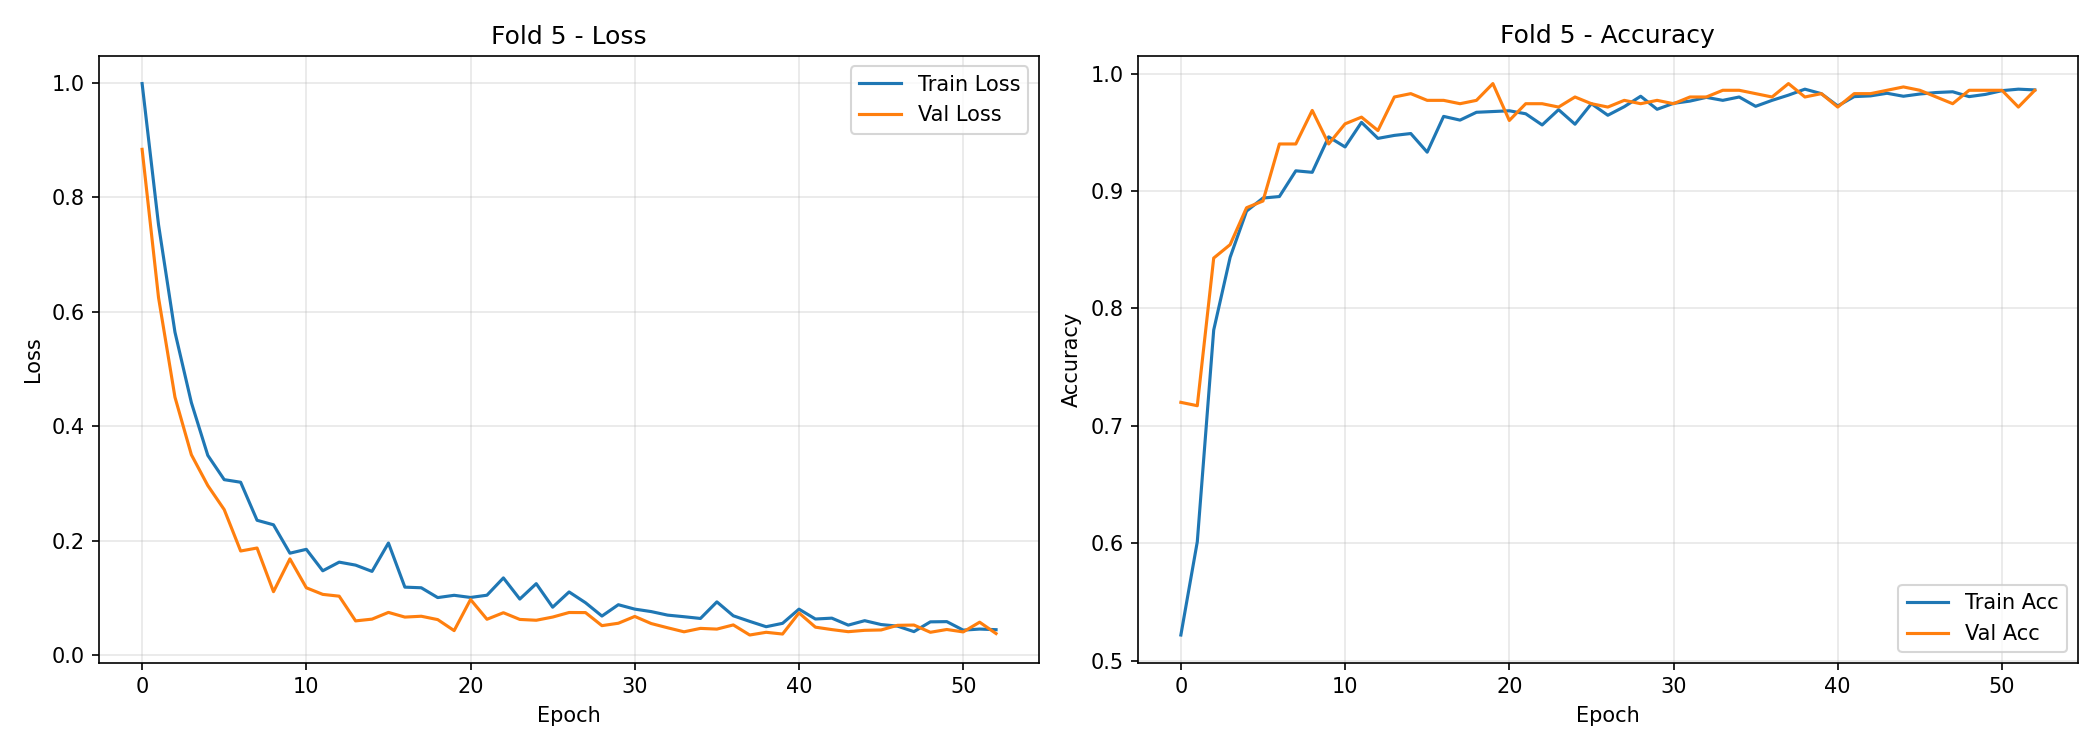
\includegraphics[width=0.82\textwidth]{figures/tc_three_fold5.png}
\vspace{0.1cm}

(c) Fold 9 --- plateaus around 94\%\\[0.1em]
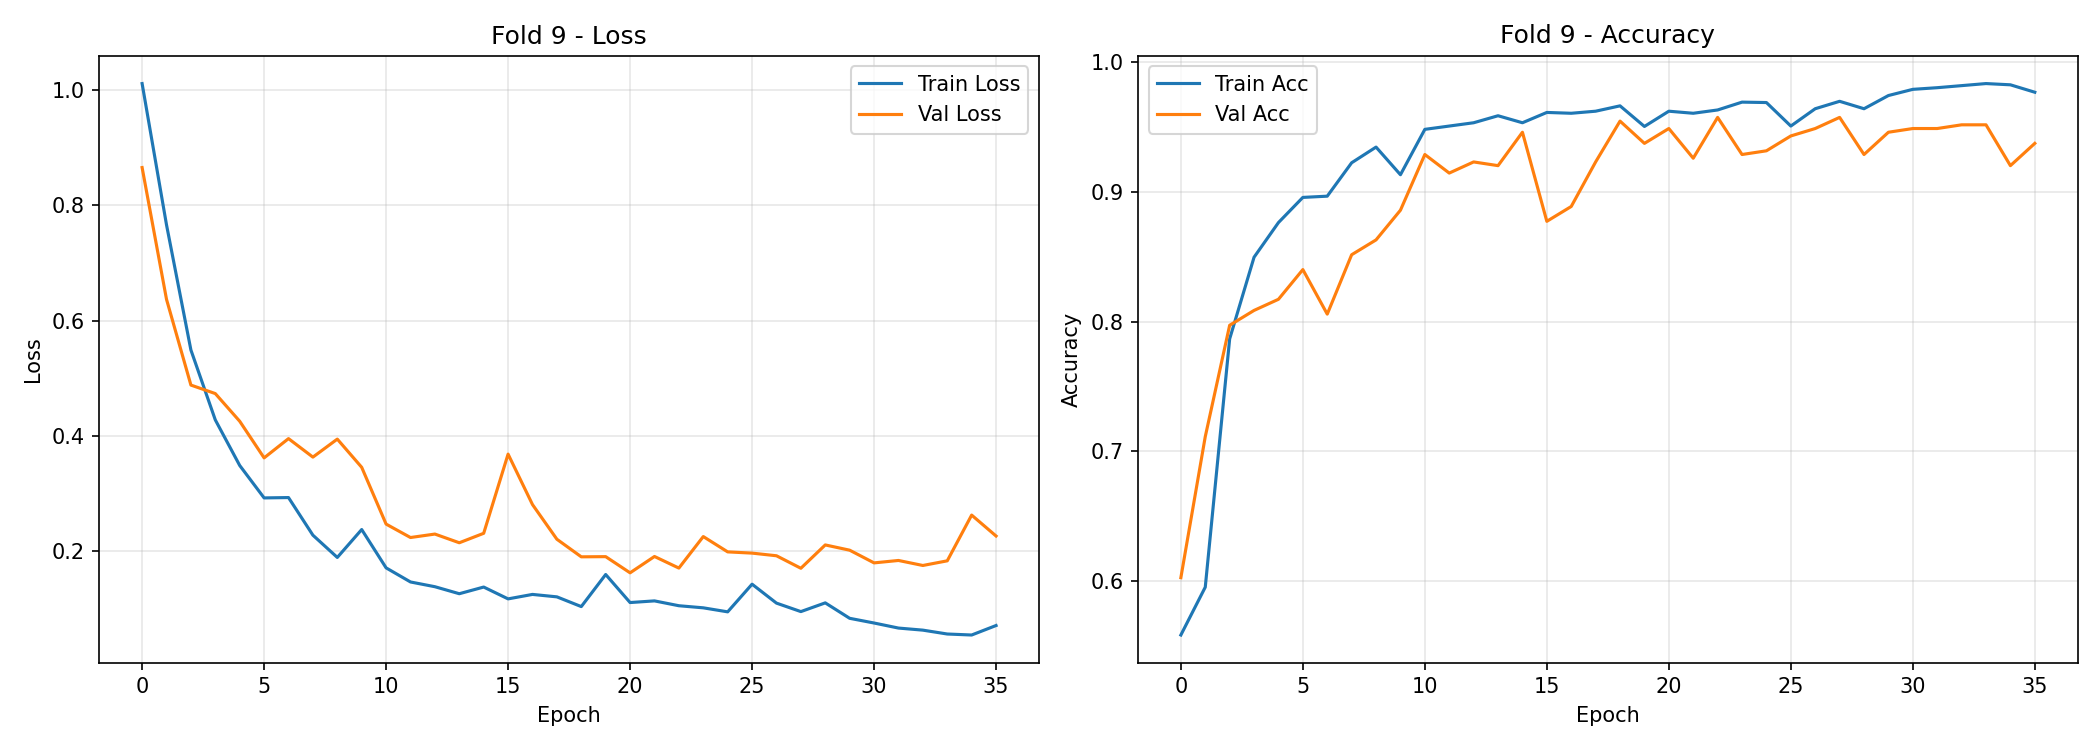
\includegraphics[width=0.82\textwidth]{figures/tc_three_fold9.png}
\vspace{0.1cm}

(d) Fold 10 --- plateaus around 95\%\\[0.1em]
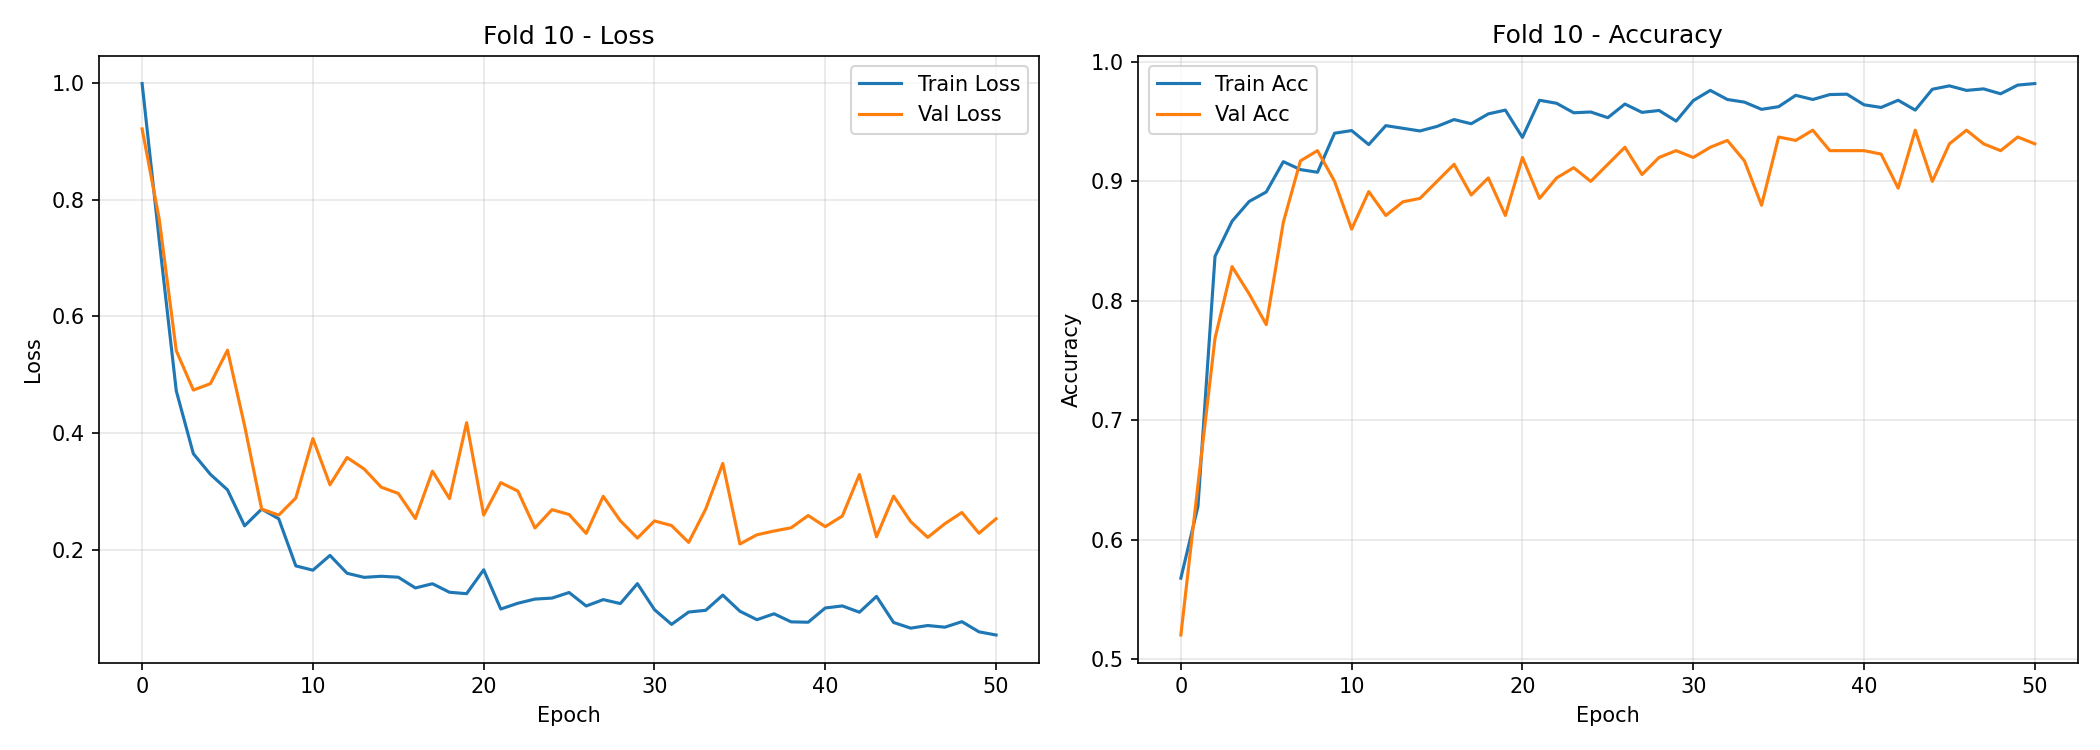
\includegraphics[width=0.82\textwidth]{figures/tc_three_fold10.png}
\caption{Three-class training curves --- representative individual folds. (a)(b) high-performing folds converging above 97\%; (c)(d) lower-performing folds plateauing around 94--95\%.}
\label{fig:tc_three_fold}
\end{figure}

\subsubsection{Five-class Classification: Z vs.\ O vs.\ N vs.\ F vs.\ S}

Table~\ref{table:five_results} presents the most challenging task. The five-class task requires the model to distinguish between physiologically similar subsets, particularly between N and F (both inter-ictal recordings from different brain regions) and between Z and O (both normal recordings under different eye conditions).

\begin{table}[H]
  \centering
  \begin{spacing}{1.35}
  \caption{Five-class Classification Results --- Z vs.\ O vs.\ N vs.\ F vs.\ S}\vspace{0.7em}
  \label{table:five_results}
    {\small
    \begin{tabular}{|>{\raggedright\arraybackslash}p{7.0cm}|>{\raggedright\arraybackslash}p{2.8cm}|>{\raggedright\arraybackslash}p{2.8cm}|}
    \hline
    \textbf{Model} & \textbf{Accuracy (\%)} & \textbf{F1 Score (\%)} \\
    \hline
    SVM + Wavelet Packet & 78.80 ($\pm$5.31) & 78.39 ($\pm$5.69) \\
    \hline
    Pure 1D-CNN & 78.86 ($\pm$3.77) & 75.95 ($\pm$5.12) \\
    \hline
    Pure Bi-LSTM + Attention & 73.09 ($\pm$8.37) & 71.92 ($\pm$9.24) \\
    \hline
    \textbf{CNN + Bi-LSTM + Attention (Ours)} & \textbf{84.51 ($\pm$3.62)} & \textbf{84.28 ($\pm$3.80)} \\
    \hline
    \end{tabular}
    }
  \end{spacing}
\end{table}

The hybrid model achieves 84.51\% accuracy, outperforming Pure CNN by +5.65\%, SVM by +5.71\%, and Pure Bi-LSTM by +11.42\%. The hybrid model also exhibits the lowest standard deviation ($\pm$3.62\%) among the deep learning models, indicating the lowest cross-fold variance in this task.

Figure~\ref{fig:tc_five_combined} shows the combined 10-fold training curves. Convergence takes longer than binary or three-class (typically 40--60 epochs), and the spread between folds is noticeably wider, consistent with the $\pm$3.62\% standard deviation in Table~\ref{table:five_results}.

\begin{figure}[H]
\centering
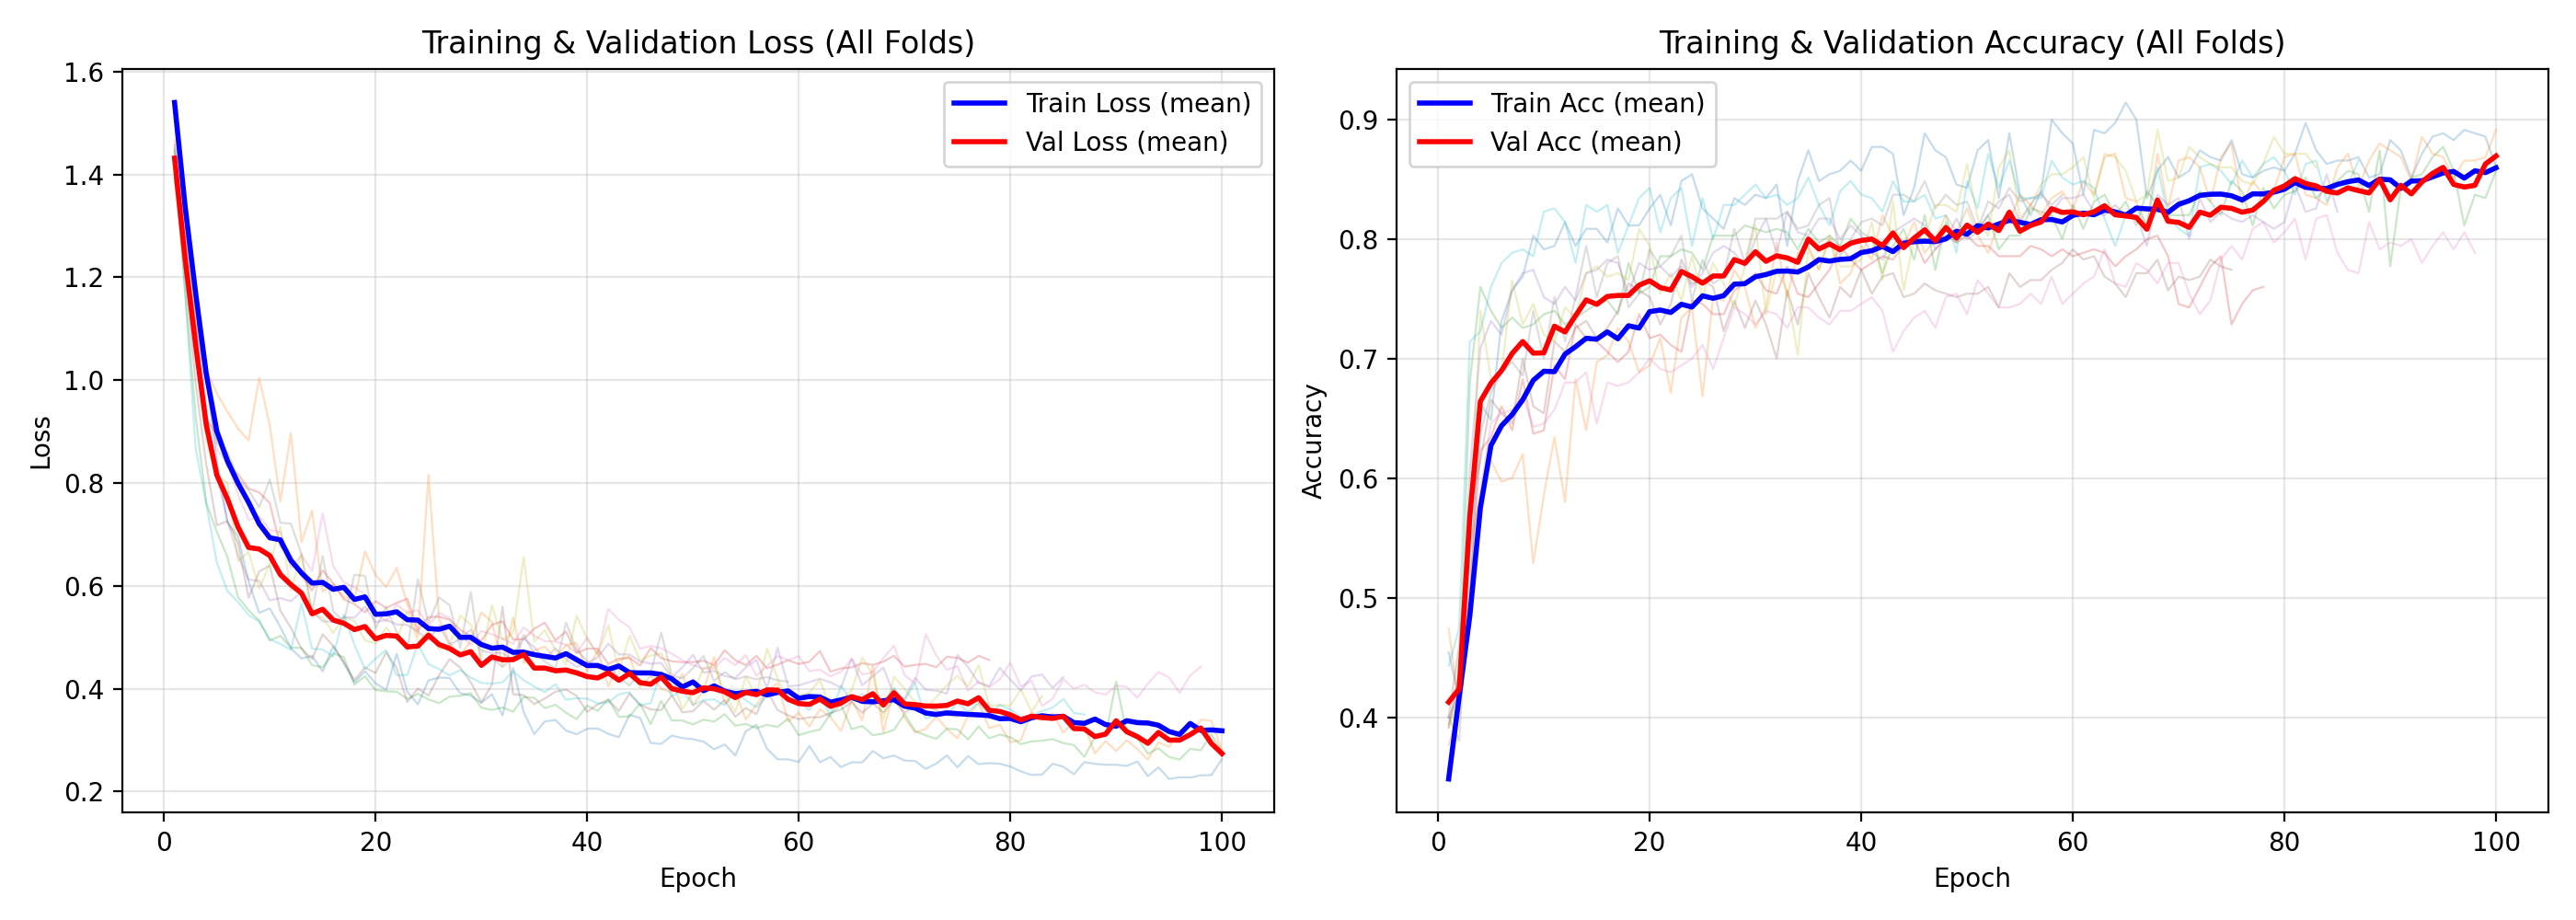
\includegraphics[width=\textwidth]{figures/training_curves_five_hybrid.png}
\caption{Combined 10-fold training curves for five-class classification. The wider spread between folds reflects the greater difficulty of this task.}
\label{fig:tc_five_combined}
\end{figure}

Figure~\ref{fig:tc_five_fold} compares Fold~1 (88.9\%, one of the best) with Fold~4 (78.9\%, one of the worst). The 10\% gap illustrates how recording-level data partitions can affect five-class performance, particularly the N/F separation.

\begin{figure}[H]
\centering
(a) Fold 1 --- best performance (88.9\%)\\[0.2em]
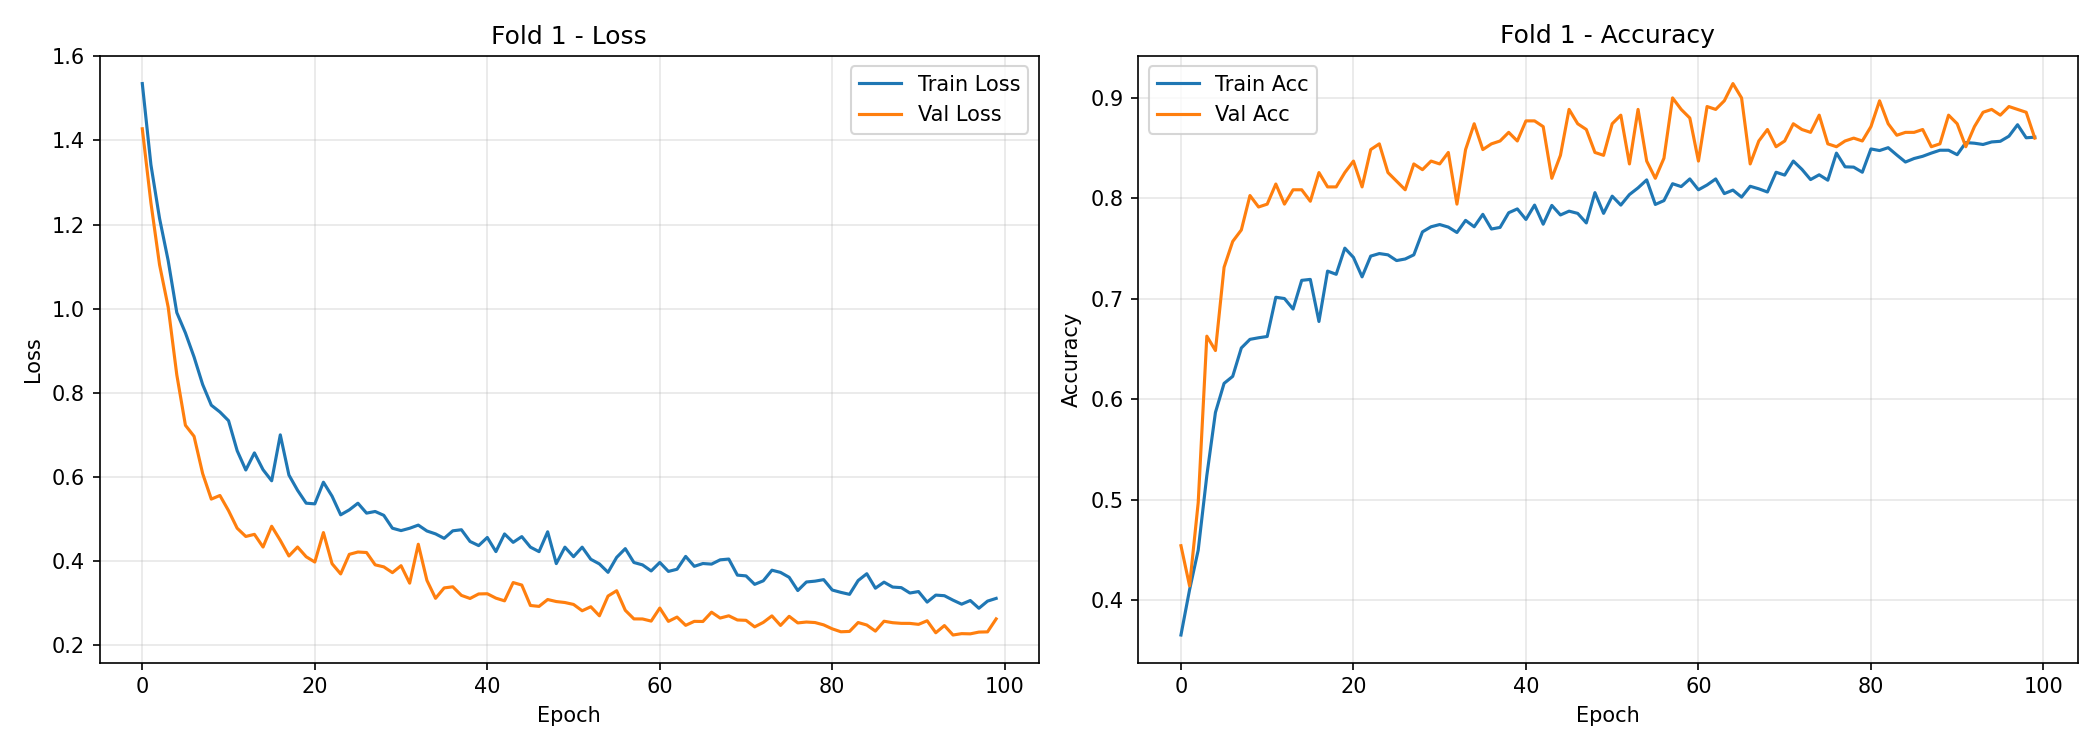
\includegraphics[width=0.88\textwidth]{figures/tc_five_fold1.png}
\vspace{0.15cm}

(b) Fold 4 --- lowest performance (78.9\%)\\[0.2em]
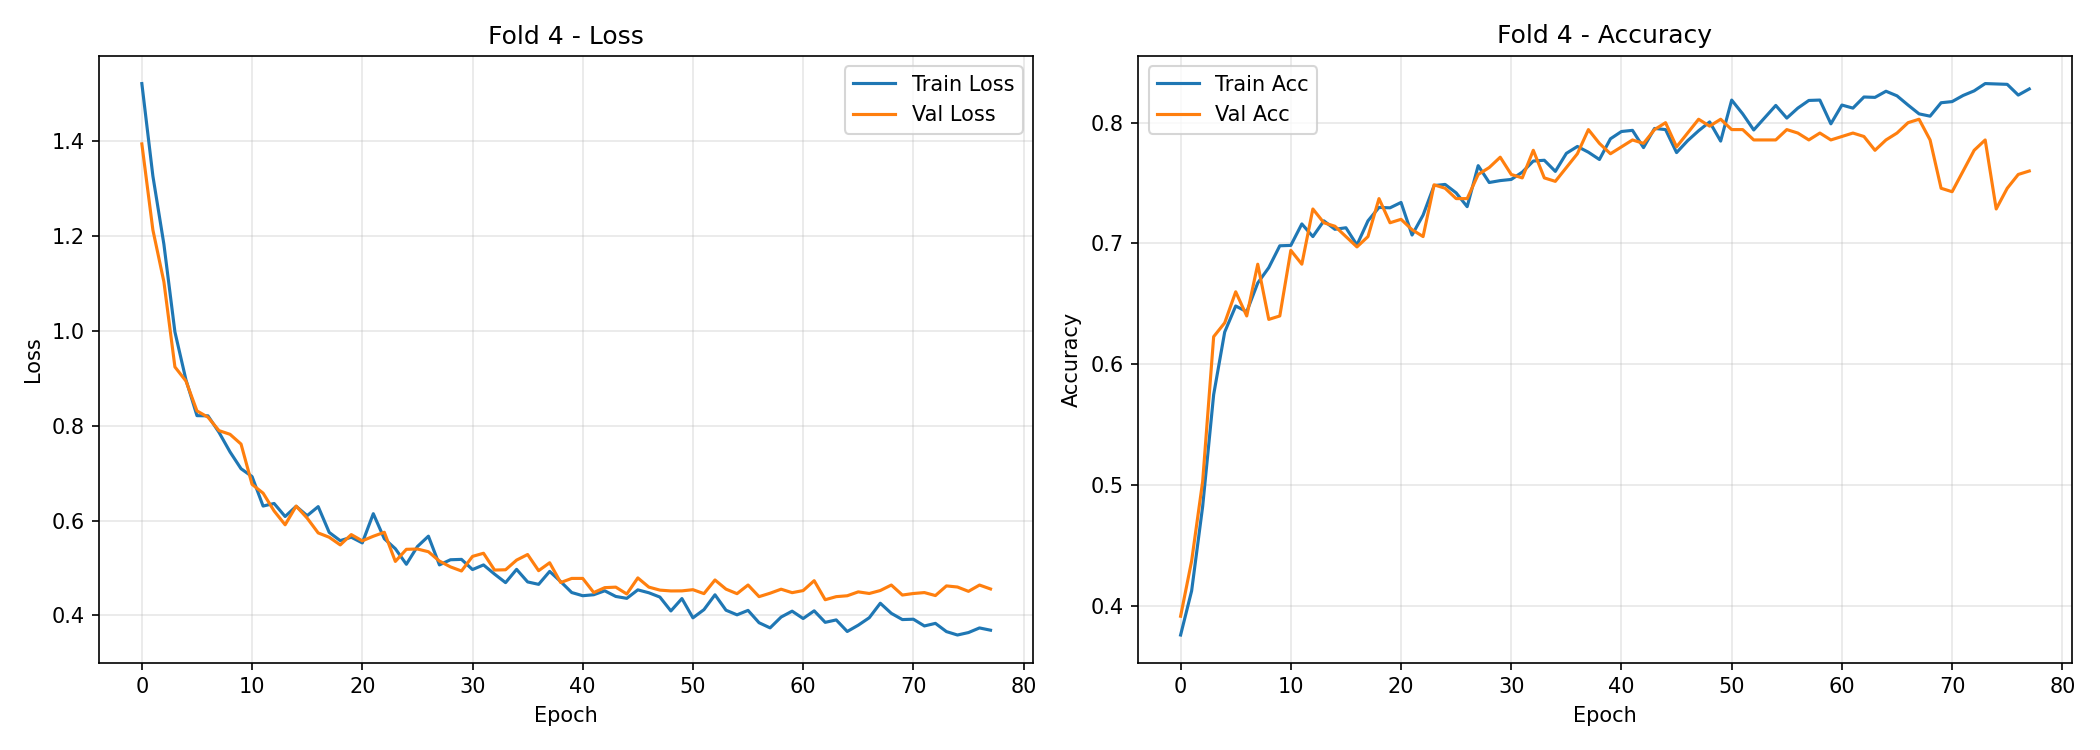
\includegraphics[width=0.88\textwidth]{figures/tc_five_fold4.png}
\caption{Individual fold training curves for five-class classification, showing the best and worst folds.}
\label{fig:tc_five_fold}
\end{figure}

\subsection{Confusion Matrix and Error Pattern Analysis}

Figure~\ref{fig:cm_binary} shows the aggregated confusion matrix for the hybrid model on binary classification. The result is near-perfect: out of all test samples across 10 folds, only a handful of seizure samples were misclassified as normal. This confirms the ceiling effect discussed in Section~4.1.1.

\begin{figure}[H]
\centering
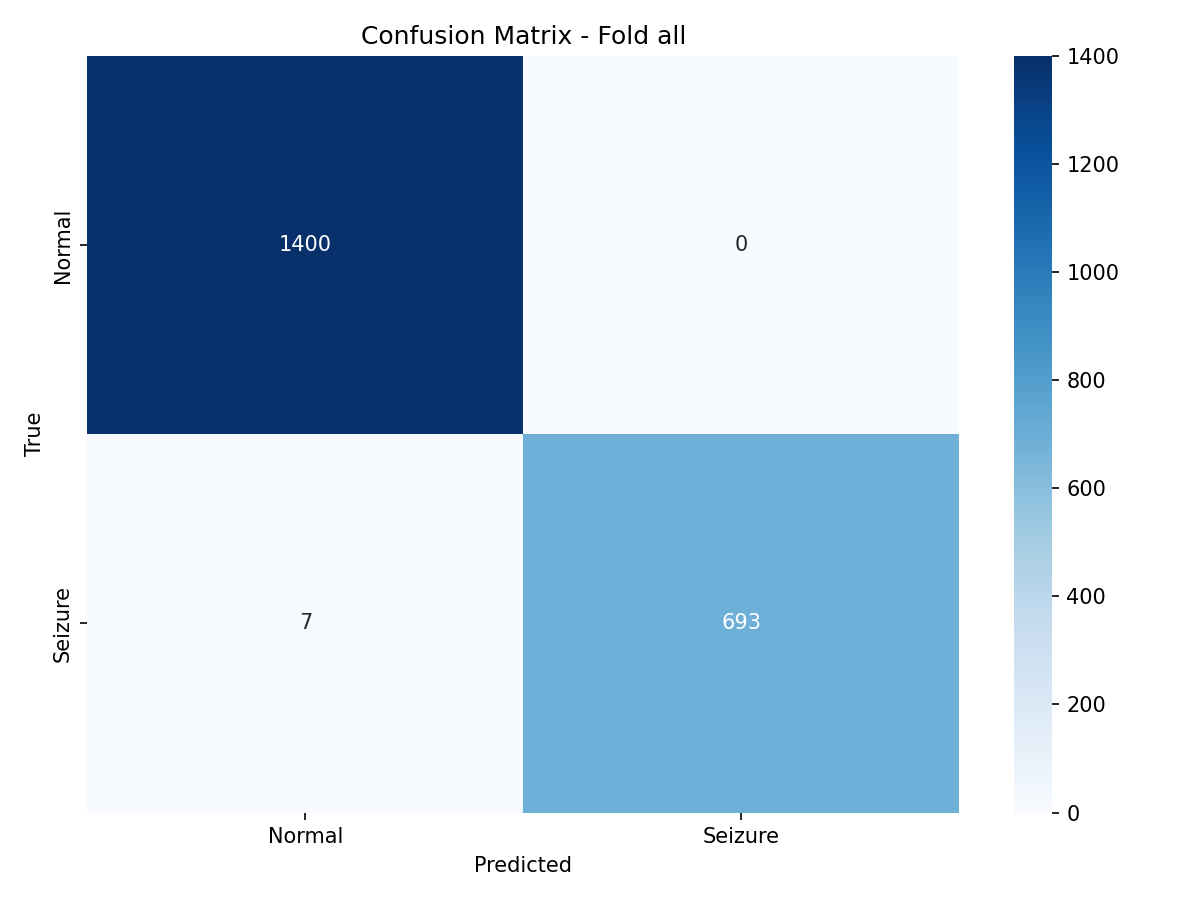
\includegraphics[width=0.6\textwidth]{figures/cm_binary_hybrid.png}
\caption{Aggregated confusion matrix for the hybrid model on binary classification (Normal vs.\ Seizure)}
\label{fig:cm_binary}
\end{figure}

Figure~\ref{fig:cm_three} shows the three-class result. The model separates all three classes well, though a small number of inter-ictal samples are confused with the normal class.

\begin{figure}[H]
\centering
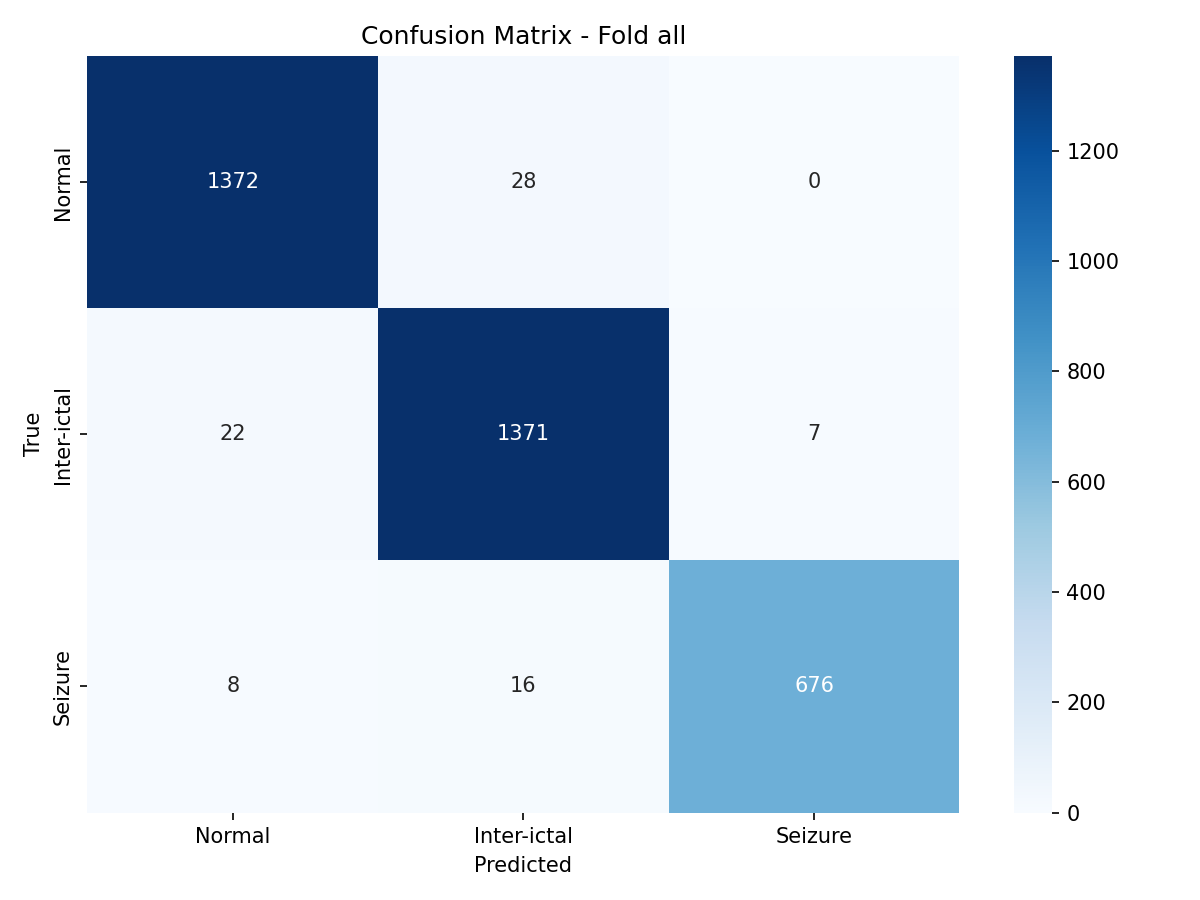
\includegraphics[width=0.65\textwidth]{figures/cm_three_hybrid.png}
\caption{Aggregated confusion matrix for the hybrid model on three-class classification}
\label{fig:cm_three}
\end{figure}

The five-class task (Figure~\ref{fig:cm_five_hybrid}) reveals the primary error source: \textbf{confusion between Set~N and Set~F}. Both subsets contain inter-ictal EEG recordings from epilepsy patients --- Set~N from the hippocampal formation contralateral to the epileptogenic zone, and Set~F from within the epileptogenic zone itself. Their physiological similarity makes them difficult to distinguish and is likely a major reason why five-class performance remains well below binary performance. A secondary source of error is mild confusion between Set~Z (eyes open) and Set~O (eyes closed), which differ mainly in the presence or absence of the alpha rhythm. In contrast, Set~S (seizure) is almost never misclassified.

\begin{figure}[H]
\centering
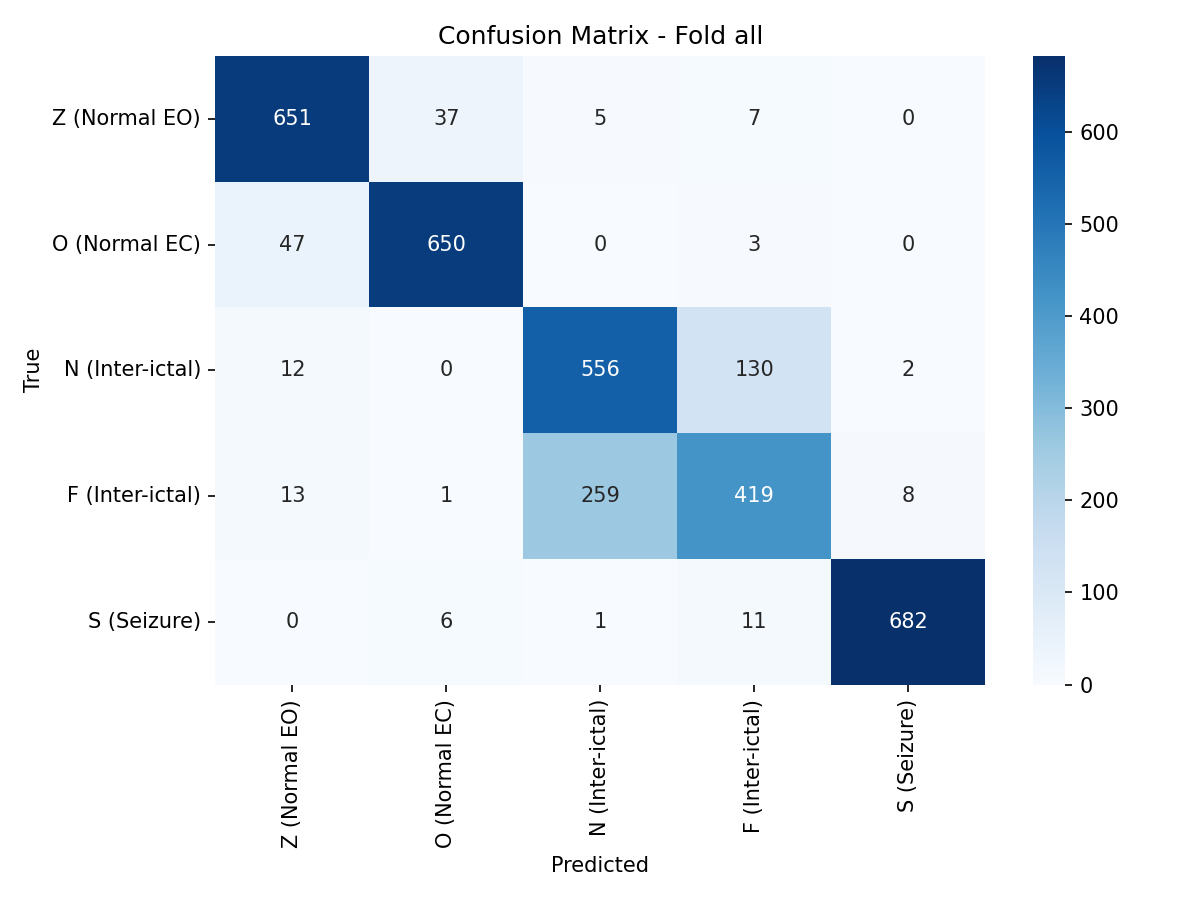
\includegraphics[width=0.7\textwidth]{figures/cm_five_hybrid.png}
\caption{Aggregated confusion matrix for the hybrid model on five-class classification. The N$\leftrightarrow$F confusion is the dominant error source.}
\label{fig:cm_five_hybrid}
\end{figure}

To understand how the baselines differ, Figure~\ref{fig:cm_five_baselines} compares the five-class confusion matrices of all four models. The SVM and Pure CNN show similar overall patterns to the hybrid model but with more errors spread across the off-diagonal cells. The Pure Bi-LSTM shows notably worse separation --- its N and F columns are heavily confused, and even the Z/O distinction degrades. The hybrid model achieves the cleanest diagonal, particularly for the N and F classes where CNN-based local feature extraction appears to be important.

\begin{figure}[H]
\centering
\begin{minipage}{0.48\textwidth}
    \centering
    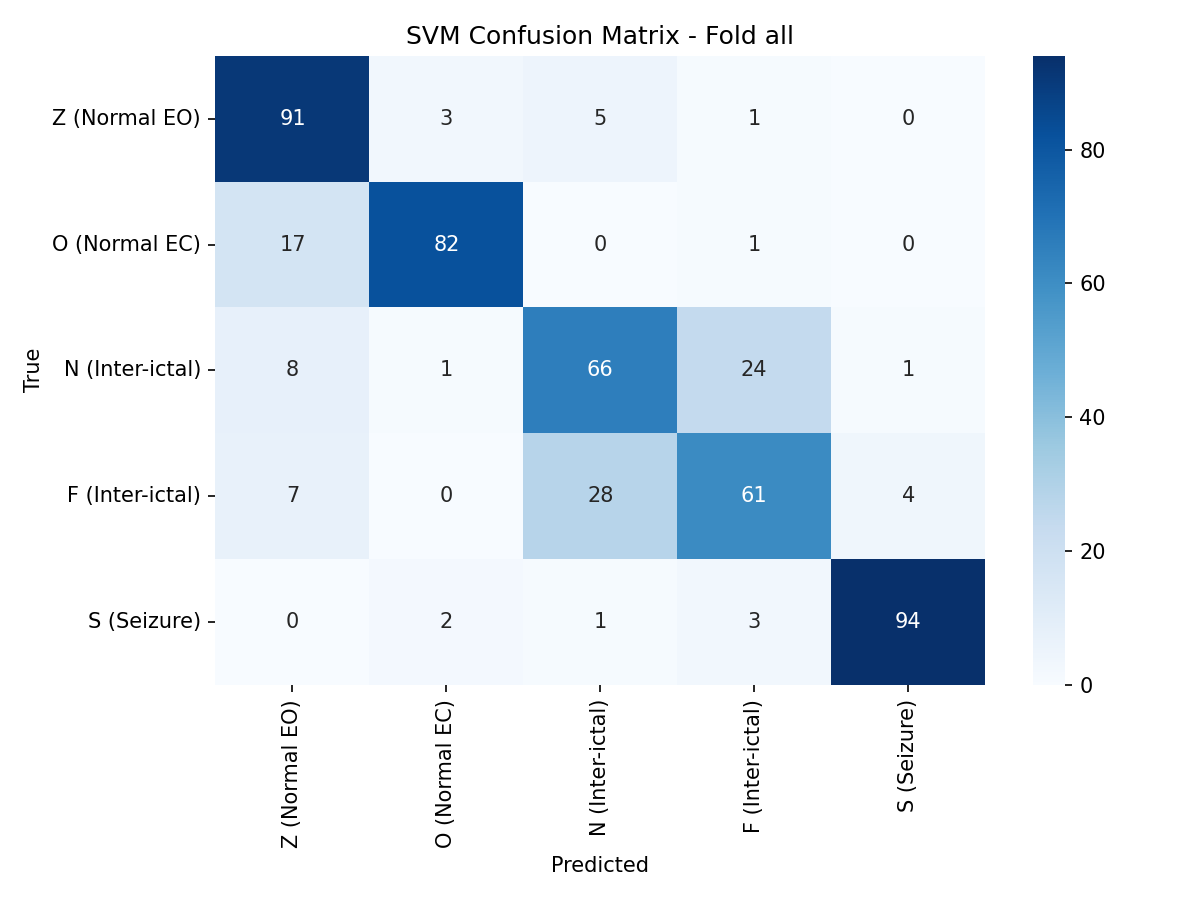
\includegraphics[width=\textwidth]{figures/cm_five_svm.png}
    \par\small (a) SVM + Wavelet Packet
\end{minipage}\hfill
\begin{minipage}{0.48\textwidth}
    \centering
    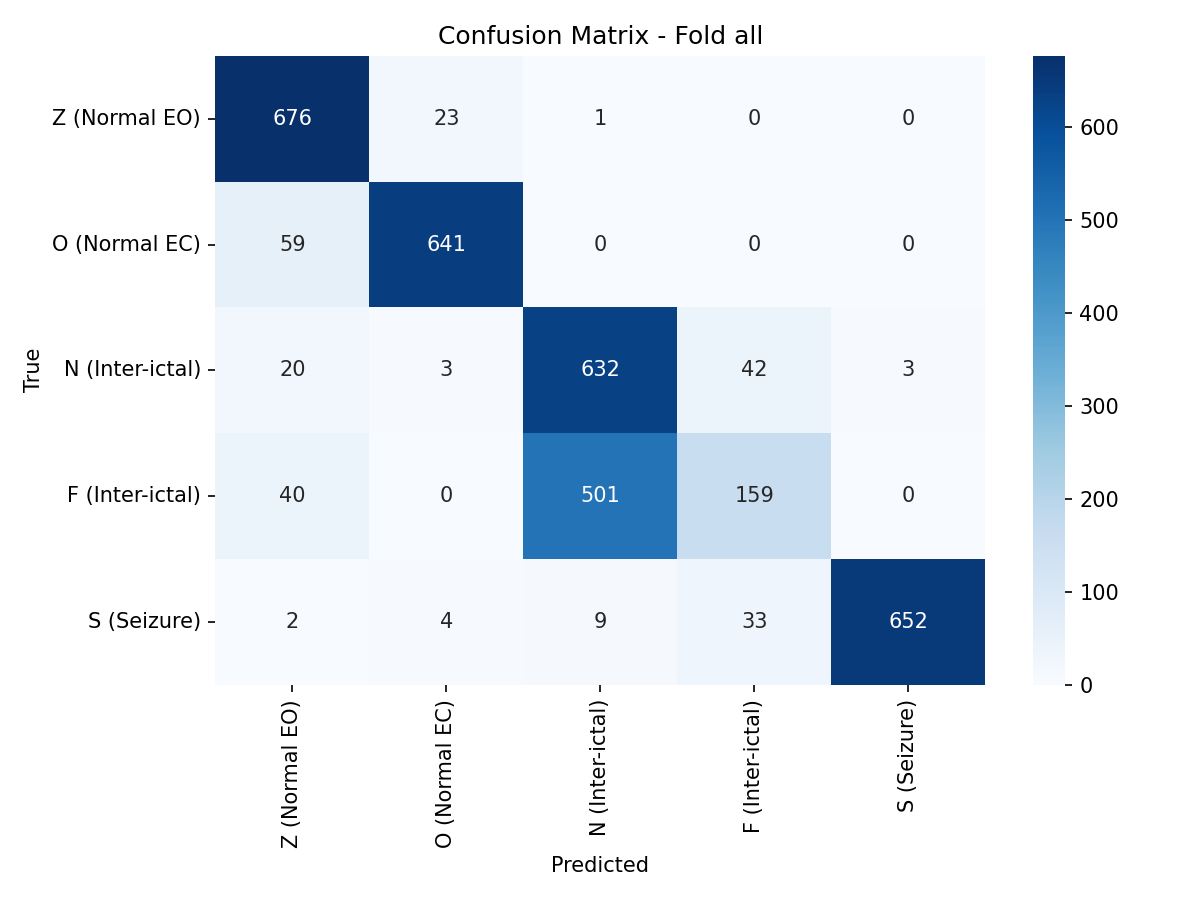
\includegraphics[width=\textwidth]{figures/cm_five_cnn.png}
    \par\small (b) Pure 1D-CNN
\end{minipage}

\vspace{0.5cm}

\begin{minipage}{0.48\textwidth}
    \centering
    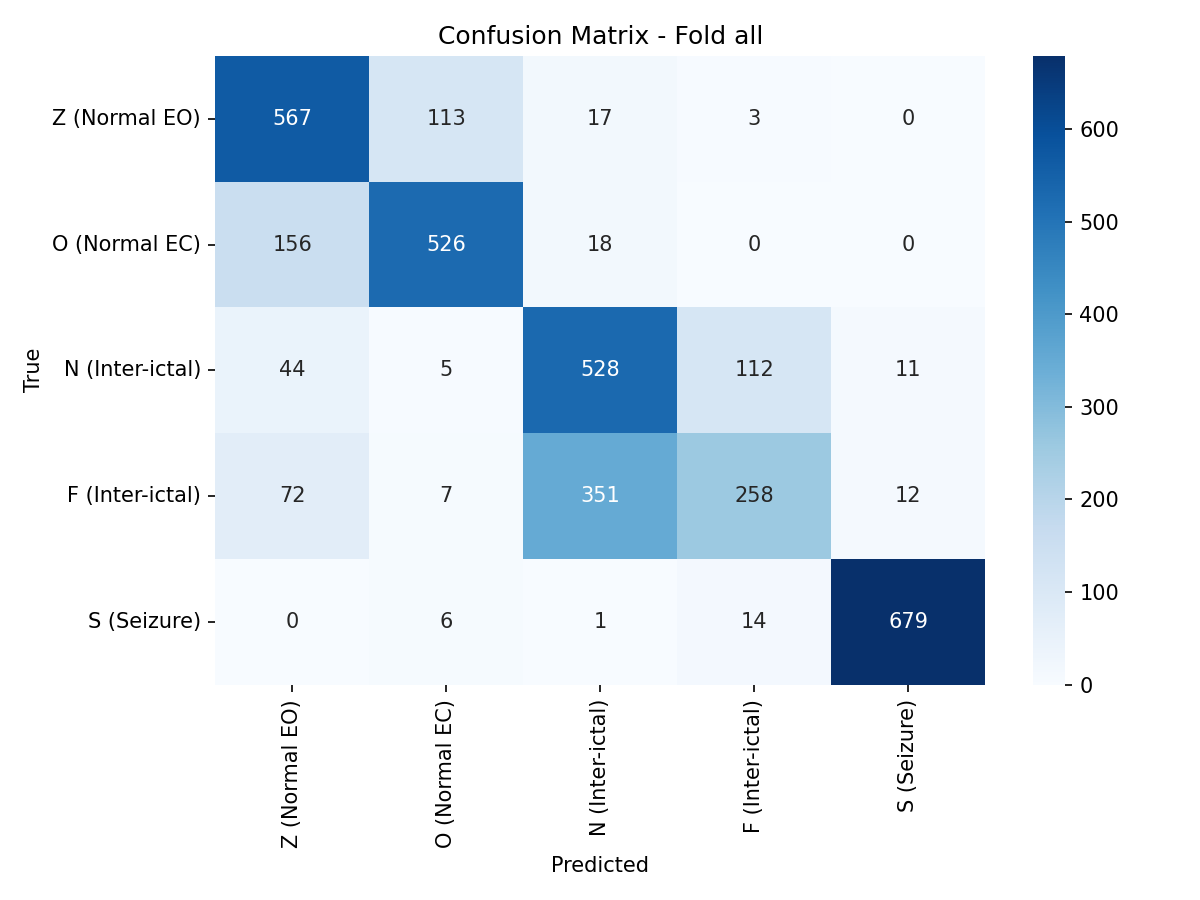
\includegraphics[width=\textwidth]{figures/cm_five_bilstm.png}
    \par\small (c) Pure Bi-LSTM + Attention
\end{minipage}\hfill
\begin{minipage}{0.48\textwidth}
    \centering
    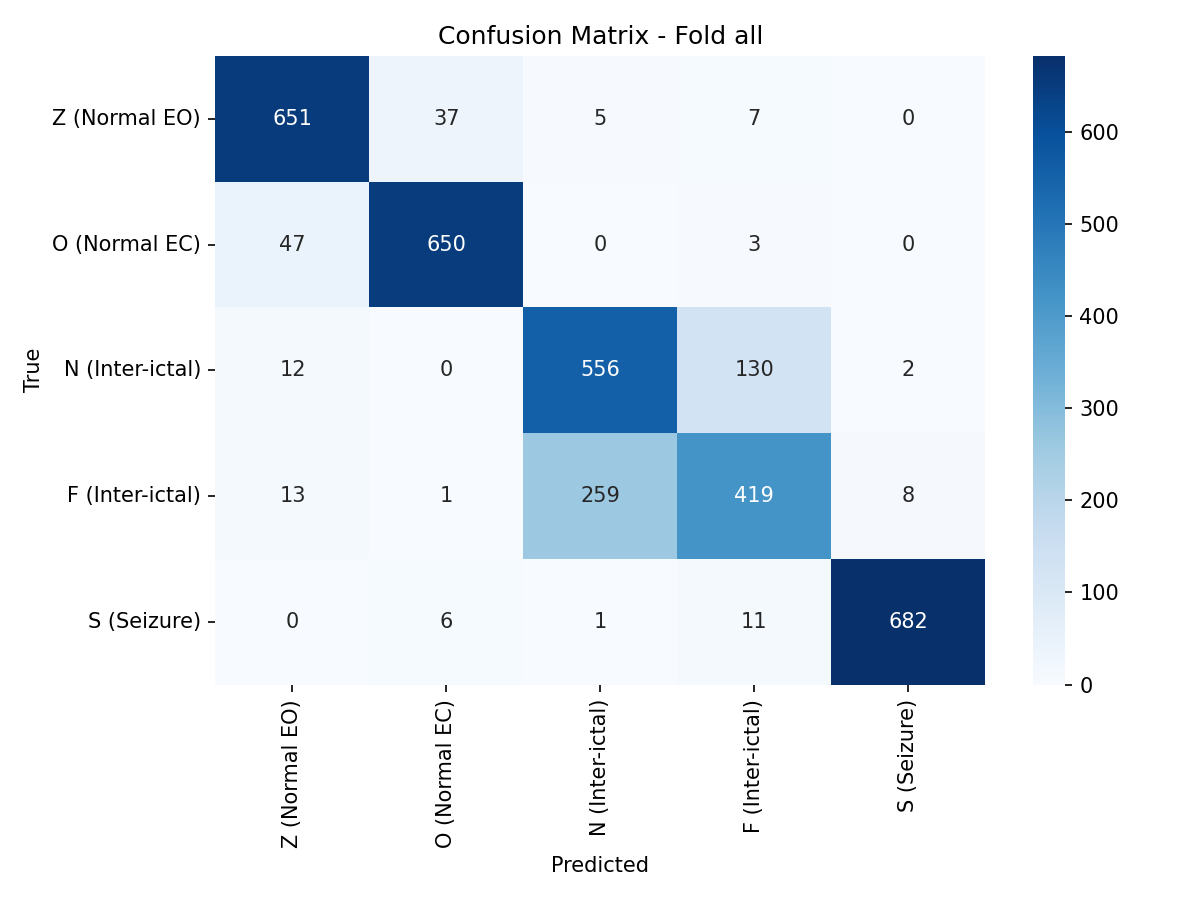
\includegraphics[width=\textwidth]{figures/cm_five_hybrid.png}
    \par\small (d) Hybrid (Ours)
\end{minipage}
\caption{Comparison of five-class confusion matrices across all four models. The hybrid model (d) shows the cleanest diagonal with fewest off-diagonal errors.}
\label{fig:cm_five_baselines}
\end{figure}

\subsection{Attention Weight Visualisation and Interpretability}

To investigate the interpretability of the proposed model, the learned Self-Attention weights were extracted and visualised for several representative EEG recordings. Figure~\ref{fig:attention_heatmap} shows the attention weight distribution overlaid on the normalised EEG signal for four representative recordings.

\begin{figure}[H]
\centering
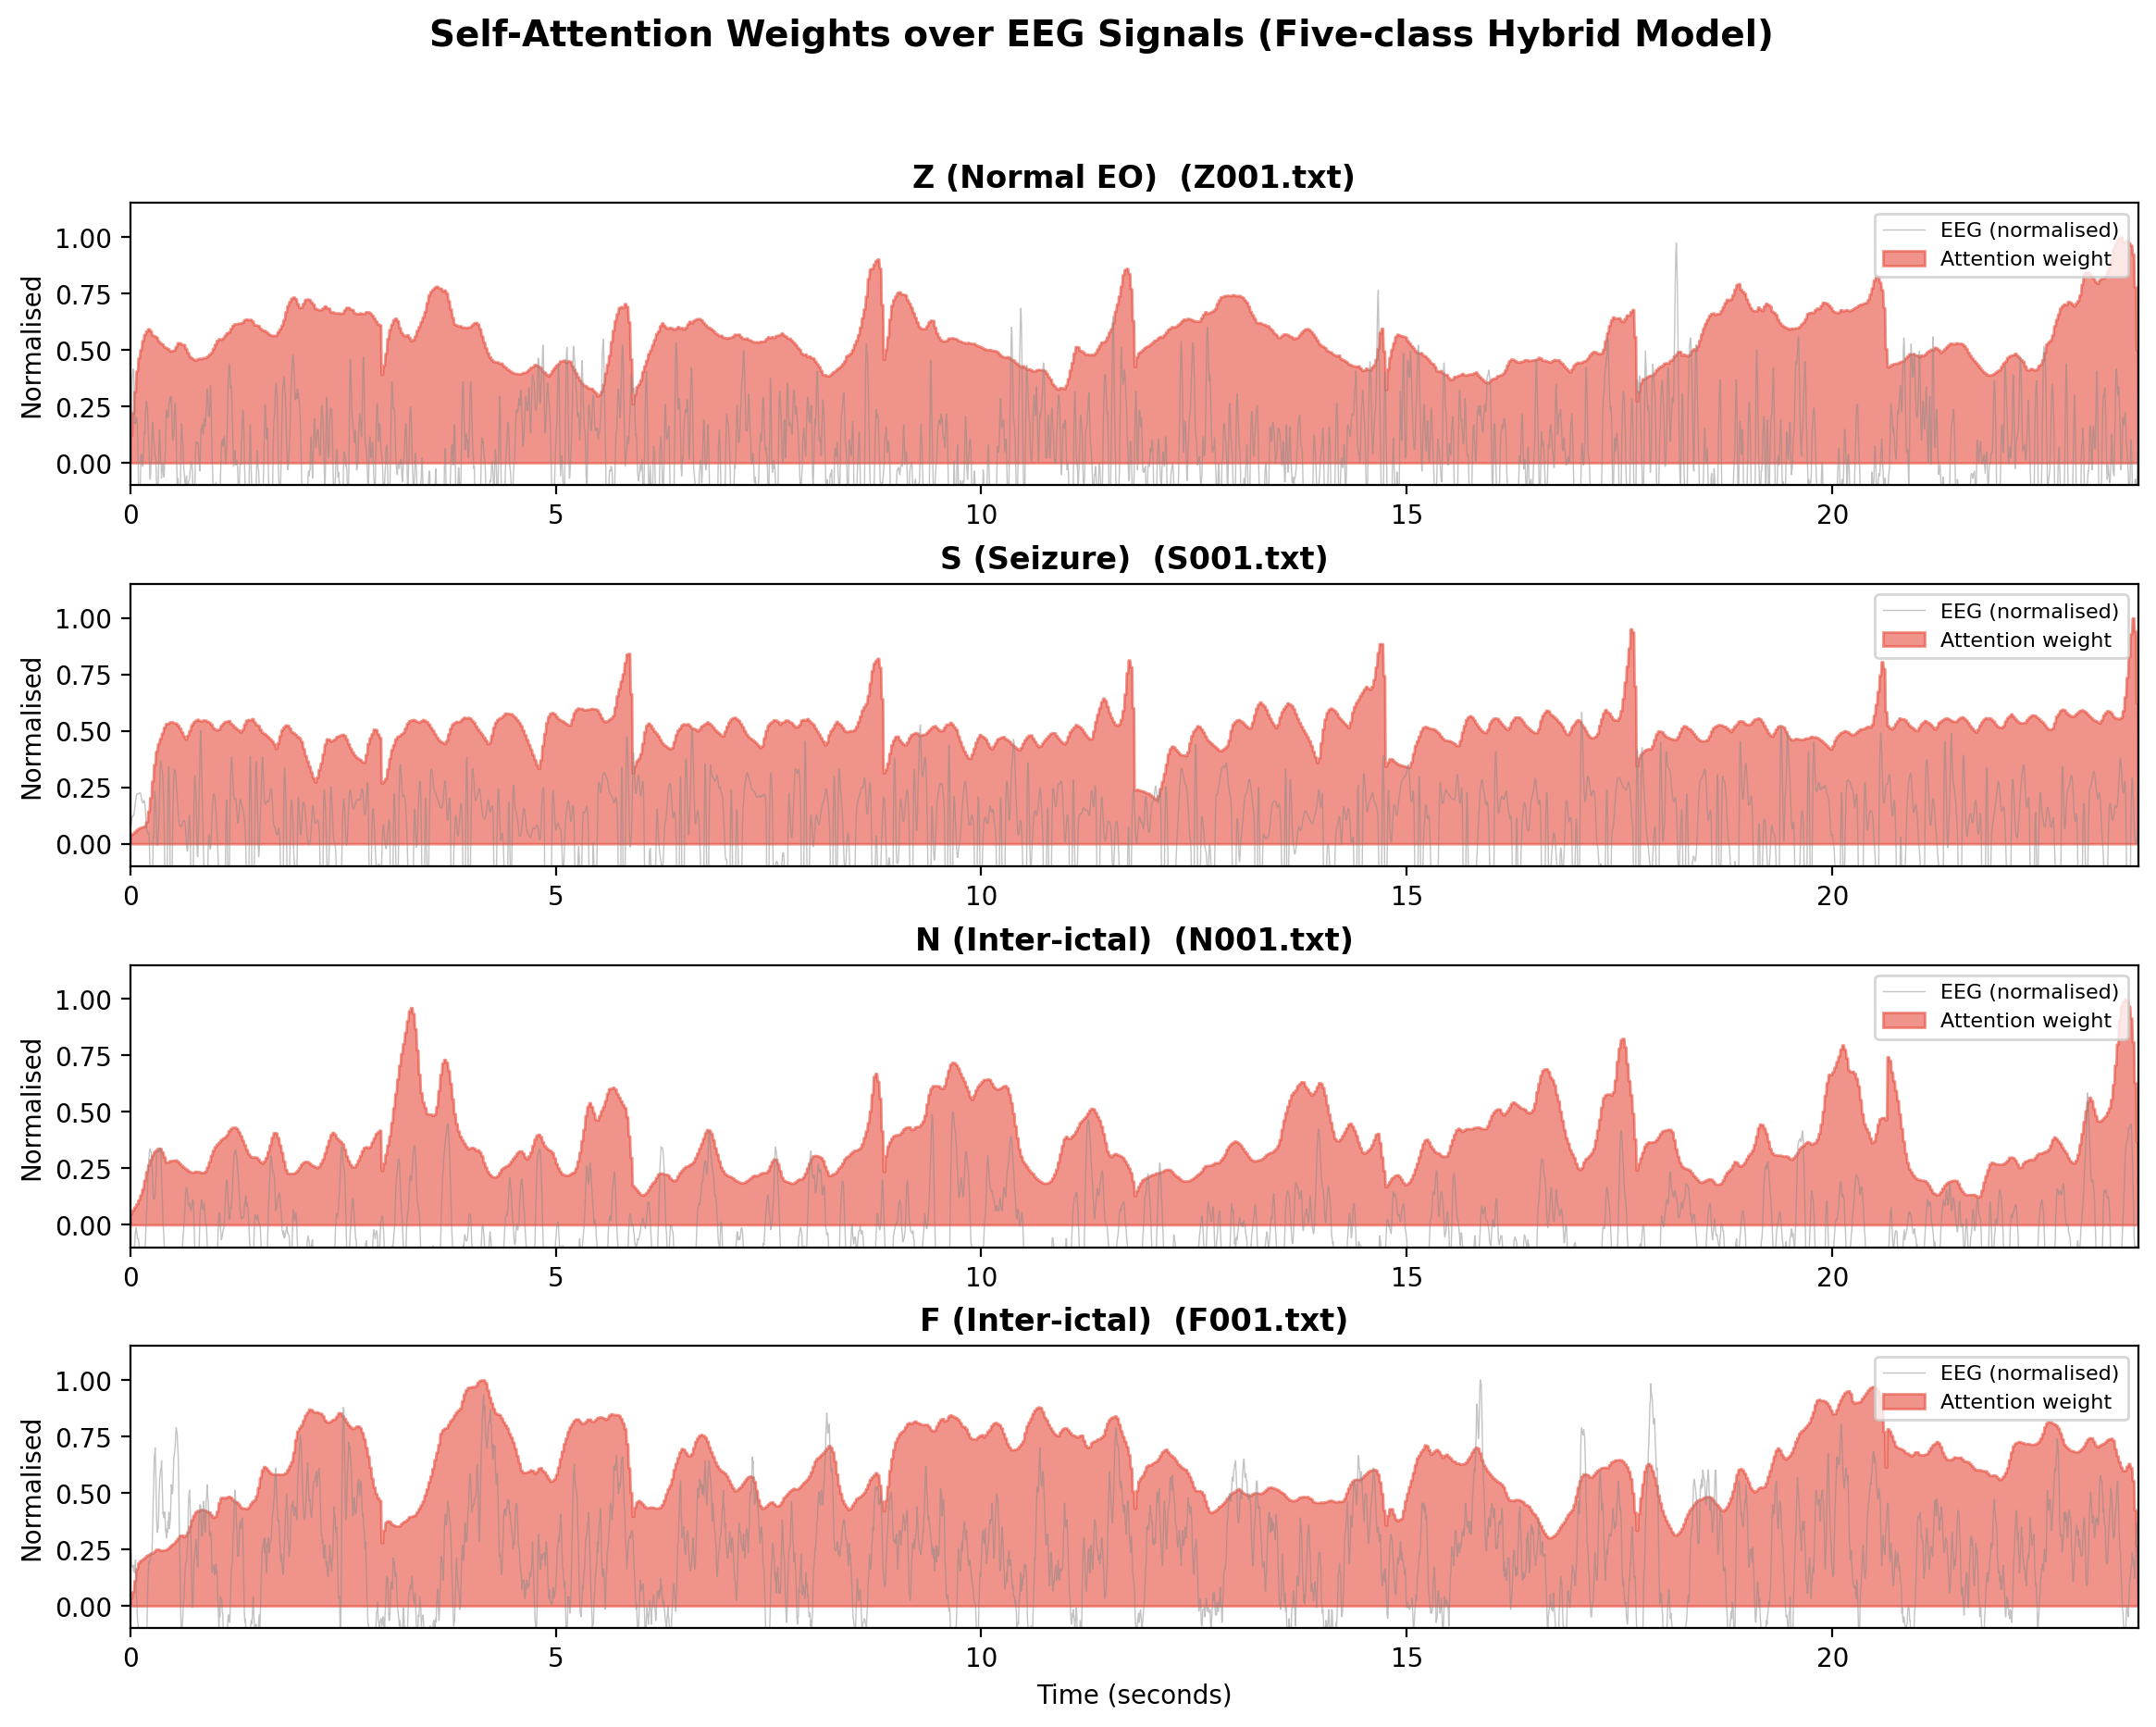
\includegraphics[width=\textwidth]{figures/attention_heatmap.png}
\caption{Self-Attention weight visualisation for representative EEG recordings from the five-class hybrid model. The normalised EEG signal is shown in grey, with attention weights overlaid in red. Higher red intensity indicates greater model focus on that temporal region.}
\label{fig:attention_heatmap}
\end{figure}

The visualisation reveals distinct attention patterns across different EEG classes:

\begin{itemize}
    \item \textbf{Seizure recordings (S)}: Attention is concentrated on the high-amplitude, rhythmic discharge regions, which are the hallmark of ictal activity. This aligns with the clinical criteria used by neurologists for seizure identification.
    \item \textbf{Normal recordings (Z)}: Attention is distributed more uniformly across the signal, reflecting the absence of pathological transients.
    \item \textbf{Inter-ictal recordings (N, F)}: Attention shows intermediate patterns, with occasional peaks corresponding to interictal epileptiform discharges (IEDs).
\end{itemize}

These patterns are consistent with the idea that the Self-Attention mechanism assigns higher weights to salient temporal regions. However, the visualisation should be interpreted as qualitative evidence about model behaviour rather than as a clinically validated explanation.

\subsection{Statistical Significance Testing}

To determine whether the observed performance differences are statistically reliable, paired t-tests were conducted across the 10 cross-validation folds for each pair of models within each task. Table~\ref{table:ttest} presents the key results.

\begin{table}[H]
  \centering
  \begin{spacing}{1.35}
  \caption{Paired t-test Results (Selected Comparisons)}\vspace{0.7em}
  \label{table:ttest}
    {\small
    \begin{tabular}{|>{\raggedright\arraybackslash}p{1.7cm}|>{\raggedright\arraybackslash}p{4.4cm}|>{\raggedright\arraybackslash}p{1.7cm}|>{\raggedright\arraybackslash}p{1.6cm}|>{\raggedright\arraybackslash}p{1.8cm}|}
    \hline
    \textbf{Task} & \textbf{Comparison} & \textbf{$t$-statistic} & \textbf{$p$-value} & \textbf{Sig.?} \\
    \hline
    Binary & Hybrid vs.\ SVM & 0.000 & 1.000 & No \\
    \hline
    Binary & Hybrid vs.\ CNN & $-$1.403 & 0.194 & No \\
    \hline
    Three & Hybrid vs.\ SVM & 4.327 & \textbf{0.002} & \textbf{Yes} \\
    \hline
    Three & Hybrid vs.\ BiLSTM & $-$2.324 & \textbf{0.045} & \textbf{Yes} \\
    \hline
    Three & CNN vs.\ SVM & 3.950 & \textbf{0.003} & \textbf{Yes} \\
    \hline
    Five & Hybrid vs.\ CNN & $-$5.247 & \textbf{0.001} & \textbf{Yes} \\
    \hline
    Five & Hybrid vs.\ BiLSTM & $-$5.289 & \textbf{0.001} & \textbf{Yes} \\
    \hline
    Five & Hybrid vs.\ SVM & 2.205 & 0.055 & No \\
    \hline
    \end{tabular}
    }
  \end{spacing}
\end{table}

The statistical analysis reveals three key findings:

\begin{enumerate}
    \item \textbf{Binary task}: Among the reported pairwise tests for the binary task, no significant differences were observed ($p > 0.05$), which is consistent with the ceiling effect discussed in Section~4.1.1. In the Bonn Z+O vs.\ S setting, several reasonable approaches reach near-perfect performance.

    \item \textbf{Five-class task}: The hybrid model \textit{significantly} outperforms both the Pure CNN ($p = 0.001$) and Pure Bi-LSTM ($p = 0.001$), supporting the view that combining CNN and Bi-LSTM components improves performance beyond random variation in this setting.

    \item \textbf{Hybrid vs.\ SVM on five-class}: Despite a 5.71\% mean accuracy advantage, the difference does not reach statistical significance ($p = 0.055$). This is attributable in part to the high inter-fold variance of SVM ($\pm$5.31\%), where SVM outperformed the hybrid model on 2 out of 10 folds. A larger study would be needed before claiming a significant advantage over SVM.
\end{enumerate}

\subsection{Comparison with Published Literature}

Table~\ref{table:literature_comparison} compares the proposed model with recently published methods on the Bonn EEG dataset.

\begin{table}[H]
  \centering
  \begin{spacing}{1.35}
  \caption{Comparison with Published Literature on the Bonn Dataset}\vspace{0.7em}
  \label{table:literature_comparison}
    {\small
    \begin{tabular}{|>{\raggedright\arraybackslash}p{4.8cm}|>{\raggedright\arraybackslash}p{0.9cm}|>{\raggedright\arraybackslash}p{1.8cm}|>{\raggedright\arraybackslash}p{3.2cm}|>{\raggedright\arraybackslash}p{1.5cm}|}
    \hline
    \textbf{Method} & \textbf{Year} & \textbf{Task} & \textbf{Evaluation} & \textbf{Acc.} \\
    \hline
    Thara et al.\ \cite{thara2019} (Stacked Bi-LSTM) & 2019 & Binary & Single split (80/20) & 99.08\% \\
    \hline
    Ullah et al.\ \cite{ullah2018} (Pyramidal CNN) & 2018 & Binary / 3-class & 10-Fold CV + aug. & Up to 99.1\% \\
    \hline
    Chen et al.\ \cite{chen2023} (RF + CNN) & 2023 & Binary & 3:1 split & 98.47\% \\
    \hline
    Huang et al.\ \cite{huang2025} (STFFDA) & 2025 & 5-class & 10-Fold CV & 67.24\% \\
    \hline
    \textbf{Ours (CNN+BiLSTM+Attn)} & \textbf{2026} & \textbf{Binary} & \textbf{10-Fold recording-level} & \textbf{99.67\%} \\
    \hline
    \textbf{Ours (CNN+BiLSTM+Attn)} & \textbf{2026} & \textbf{3-class} & \textbf{10-Fold recording-level} & \textbf{97.69\%} \\
    \hline
    \textbf{Ours (CNN+BiLSTM+Attn)} & \textbf{2026} & \textbf{5-class} & \textbf{10-Fold recording-level} & \textbf{84.51\%} \\
    \hline
    \end{tabular}
    }
  \end{spacing}
\end{table}

The proposed model performs strongly on the evaluated Bonn tasks. On the five-class task, this work reports 84.51\%, which is higher than the 67.24\% reported by Huang et al.\ \cite{huang2025}. The comparison should still be read with care, because the preprocessing and sample construction differ between the two studies. Even so, the result suggests that the current hybrid pipeline remains competitive under a stricter recording-level split.

\subsection{Clinical Applicability and Limitations}

The proposed system is better viewed as a proof-of-concept for offline EEG classification than as a deployable clinical decision support tool. The strong binary result on Bonn (99.67\%) suggests that the model can separate clearly different signal classes under controlled conditions, but whether this would transfer to routine EEG monitoring remains to be tested.

The attention visualisation in Section~4.3 offers a limited interpretability signal by highlighting which temporal regions received higher weights, but this should not be treated as direct clinical validation.

However, several limitations must be acknowledged:

\begin{itemize}
    \item \textbf{Single dataset}: All experiments were conducted on the Bonn dataset, which is relatively small (500 recordings) and clean (pre-filtered, artefact-free). Performance on noisy, real-world clinical recordings may differ.
    \item \textbf{Single-channel}: The Bonn dataset contains only single-channel EEG, whereas modern clinical EEG typically uses multi-channel montages (19+ channels). The model's ability to leverage spatial information from multi-channel data remains unexplored.
    \item \textbf{Class imbalance}: The binary task involves a 2:1 class ratio (200 Normal vs.\ 100 Seizure recordings). No explicit class weighting was applied, and no clear degradation was observed in the reported binary results, but the imbalance should still be considered when generalising to more imbalanced clinical datasets.
    \item \textbf{Offline analysis}: The current system processes pre-recorded EEG segments and is not optimised for real-time streaming inference.
\end{itemize}
